\documentclass{book}

% Choose a conveniently small page size
\usepackage[paperheight = 16cm, paperwidth = 12cm, textwidth = 10cm]{ geometry }
\usepackage[english, main = italian]{babel}
\usepackage{amsmath}
\usepackage{amssymb}
\usepackage{amsthm}
\usepackage{hyperref}
\usepackage[parfill]{parskip}
\usepackage[linewidth=1pt]{mdframed}
\usepackage{graphicx}

\graphicspath{ {./images/} }

\newmdtheoremenv{example}{Esempio}{\itshape}{\itshape}
\newtheorem{remark}{Osservazione}[section]

\title{Riassunto di Data and Web Mining}
\author{Un gruppo di buon samaritani}
\date{Dicembre 2022}
\begin{document}

\frontmatter
\maketitle
$$ \textbf{Prefazione} $$
Ci scusiamo per gli eventuali errori di battitura presenti nel documento.
\\
Gli argomenti presenti in questo documento si rifanno a quelli spiegati nel corso dell'anno accademico 2022/2023.
\\
Qui dentro sono riassunti i concetti che ho ritenuto più importanti da sapere.
\\
Potremmo aver saltato qualche piccola parte di alcuni argomenti causa pigrizia, confusione o altre ragioni di cause sconosciute.
\\
Non ci assumiamo nessuna responsabilità riguardo il voto che prenderete se studiate solo da questo riassunto.
\\
A dirla tutta, non siamo delle persone responsabili in primo luogo quindi il problema non dovremmo manco porcelo.
\\
Per chi stesse studiando durante le feste natalizie: tanti auguri.
\\
Chi invece no: tanti auguri lo stesso.
\\
Potremmo aver sviluppato una forte dipendenza da caffeina: se vedete il documento non concluso, una probabile causa potrebbe essere arresto cardiaco.
\\
La seconda causa è che abbiamo trovato degli appunti migliori di questi: nel caso fosse, faremo un omaggio alla madonna per la persona che li ha scritti.
\\
Se avete letto fino a questo punto, ci scusiamo per l'inutile perdita di tempo.
$$ \textbf{BUONA LETTURA}_{mandate aiuto pls!} $$


\mainmatter
\tableofcontents

    \chapter{Introduzione}

	\section{Supervised vs Unsupervised}
		
		\begin{itemize}
			\item $\textbf{Supervised learning}$: È un approccio che è definito dall'uso di set di dati già etichettati: questi set di dati sono progettati per allenare (o "supervisionare") gli algoritmi nella classificazione dei dati o nella previsione accurata dei risultati.
				\\[1\baselineskip]
				Si parla di Supervised Learning quando è l'umano a fornire già delle etichette ai dati, in modo da dare una mano all'algoritmo nella sua fase di allenamento in quanto saprà già dall'inizio saprà quali sono i dati corretti.\\
				\\[1\baselineskip]
				L'apprendimento supervisionato può essere separato in due tipi di problemi durante il data mining: classificazione e regressione.
				\\[2\baselineskip]

			\item $\textbf{Unsupervised learning}$: Utilizza algoritmi di apprendimento automatico per analizzare e raggruppare set di dati non etichettati: questi algoritmi apprendono da soli i migliori pattern che rappresentano i dati, senza la necessità dell'intervento umano.
		\end{itemize}

	\clearpage

	\section{Regressione vs Classificazione}
		
		\begin{itemize}
			\item $\textbf{Regressione:}$ L'obiettivo principale dei problemi di regressione è quello di trovare una funzione ottimale che riesca a combinare alcune variabili $X$, dette anche $\textit{predittori}$, per produrre un valore in output, ovvero $Y$, il più preciso possibile.
				Alcuni esempi di problemi di regressione possono essere la stima dei prezzi di vendita di immobili oppure la stima della probabilità di un certo evento binario, come la probabilità di terremoti in certe regioni di un paese.
				\\[2\baselineskip]
			
			\item $\textbf{Classificazione:}$ L'altra categoria di problemi sono quelli di classificazione, ovvero problemi che richiedono di trovare una funzione che utilizza alcuni predittori $X$ per produrre in output un valore $Y$ discreto (può essere un'etichetta o una categoria).
			Un esempio di problema di classificazione può essere la categorizzazione di un sito come affidabile oppure non affidabile.
		\end{itemize}

	\clearpage

	\section{Train, Validation and Test}

		L'utilizzo di un algortimo per risolvere un certo problema prevede fondamentalmente due step: l'allenamento e la classificazione.
		È comune anche aggiungere la fase di validazione dopo la fase di allenamento, in cui è possibile, appunto, validare il modello$^{[1]}$ fornito dall'algoritmo.

			\subsection{Fase di Train}
			Il processo di allenamento dell'algoritmo consiste nel fornirgli un dataset su cui può imparare a classificare i dati (da qui il nome "Train Set") e costruire un modello ottimale sulla base di ciò che ha appreso.

			\subsection{Fase di Validation}
			Nella fase di Train, l'algoritmo impara le relazioni tra input $X$ e output $Y$.
			Per evitare di cadere nell'overfitting e avere una migliore capacità predittiva, viene dato al nostro modello dei dati che non ha mai visto e gli facciamo fare una predizione (anche questi dati devono essere già etichettati).
			\\[1\baselineskip]
			Dopo le predizioni su questi dati, verranno confrontati i risultati del modello (che denomineremo con $\hat{y}$) con le $y$ reali per vedere quanto il modello riesce a prevedere con una buona approssimazione la variabile target.
			Nel caso di performance scarse, bisogna aggiustare gli iperparametri del modello e ripartire dalla fase di train, finché il risultato ottenuto dalla fase di validation non sarà soddisfacente.
			
			\subsection{Fase di Test}
			Il processo di classificazione consiste nell'utilizzo del modello, precedentemente costruito nella fase di training, per predire le categorie o stimare i valori di nuovi dati.\\
			In questa fase viene fornito al modello un set di dati su cui valutare il modello; viene utilizzato solo dopo che il modello è stato completamente allenato.
			Il Test Set contiene dati accuratamente campionati che cercano di coprire le varie casistiche che il modello dovrà affrontare se utilizzato nel mondo reale.

		\begin{figure}[ht]
			\caption{Esempio di divisione del dataset}
			\centering
			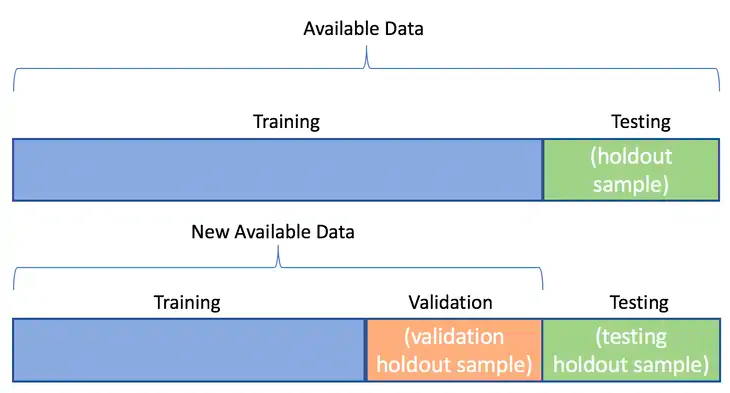
\includegraphics[width = 10cm, height = 4.2cm]{training-validation-test-split.png}
		\end{figure}

	\clearpage

	\section{Stratified Sampling}
		Il campionamento casuale generalmente va bene se il set di dati originale è sufficientemente grande proprio perché ogni sottoinsieme di $n$ istanze ha la stessa probabilità di essere selezionato come campione di qualsiasi altro sottoinsieme di $n$ istanze.
		\\
		Ma se il dataset non è sufficientemente grande, viene introdotta una distorsione a causa dell'errore di campionamento.
		\\[1\baselineskip]
		Il $\textbf{Stratified Sampling}$ è un metodo di campionamento che riduce l'errore di campionamento nei casi in cui la popolazione può essere suddivisa in sottogruppi:
		la popolazione viene divisa in sottogruppi omogenei, chamati $\textit{strati}$, per poi applicare il campionamento casuale semplice all'interno di ciascun sottogruppo.
		
		\begin{figure}[h]
			\caption{Esempio di Stratified Sampling}
			\centering
			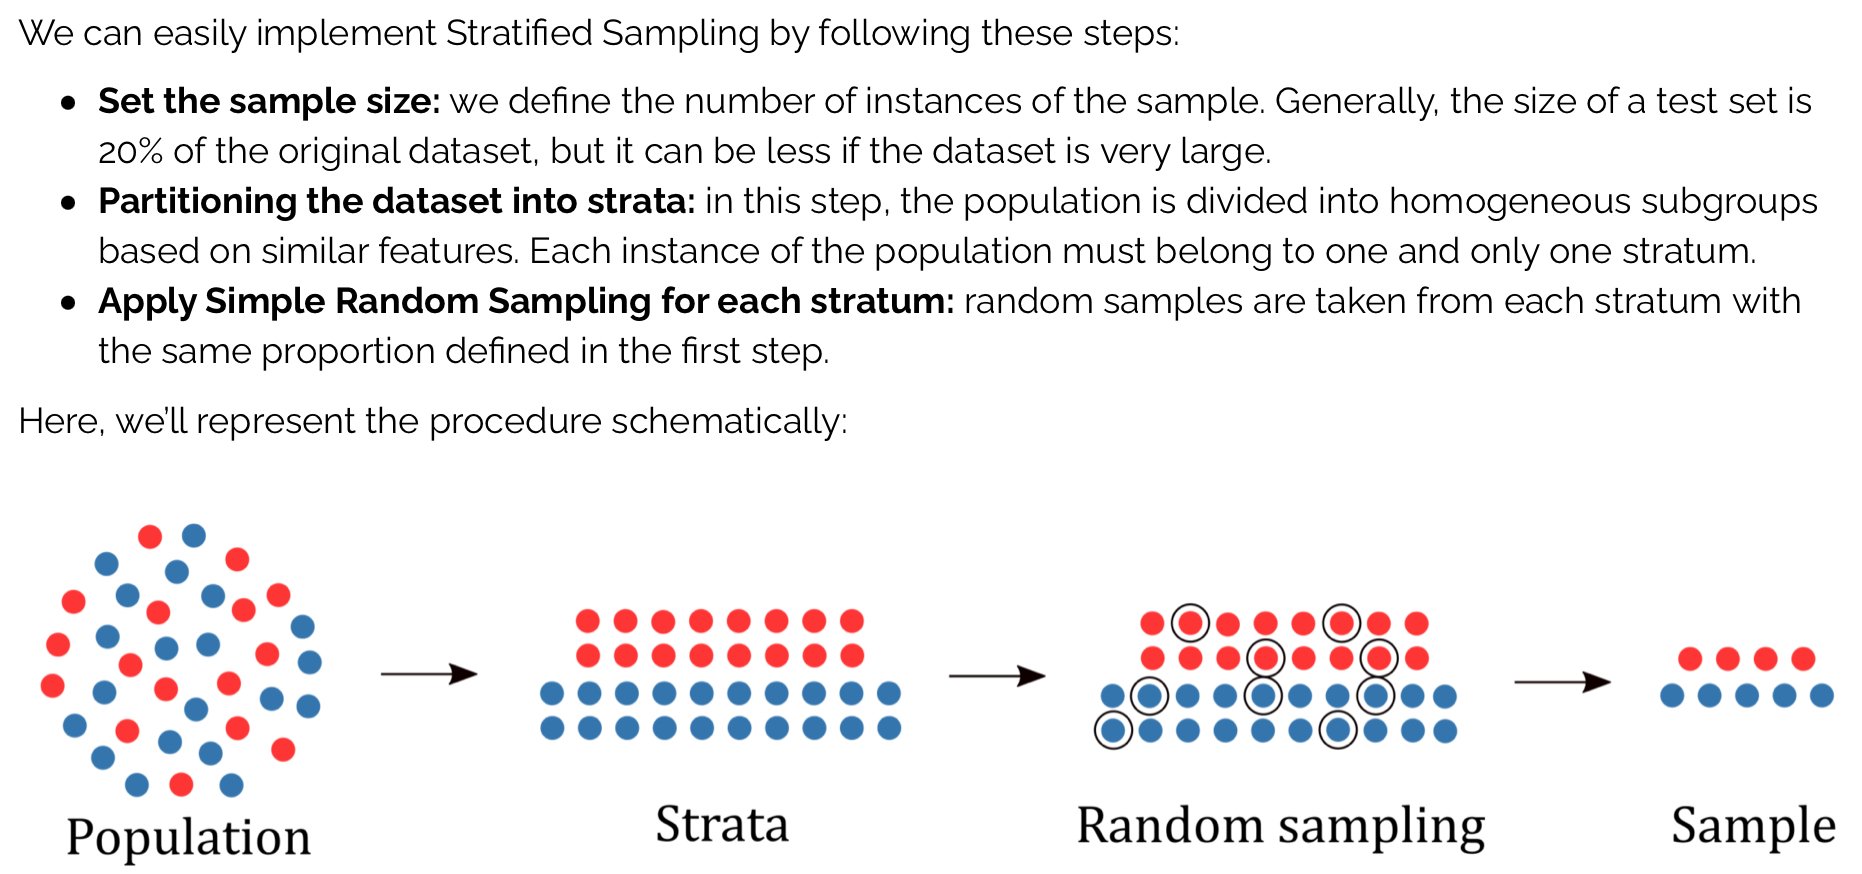
\includegraphics[width = 10cm, height = 4.2cm]{stratified-sampling-example.jpg}
		\end{figure}

	\clearpage

	\section{Cross-Validation}
		Il $\textbf{Cross-Validation}$ è una procedura di ricampionamento utilizzata per valutare i modelli di machine learning su un campione di dati limitato.
		La procedura ha un singolo parametro, ovvero $k$, che si riferisce al numero di gruppi in cui deve essere suddiviso un dato campione di dati.
		\\
		Pertanto, la procedura viene spesso chiamata
		\\
		$\textbf{K-Fold Cross-Validation}$.

		\subsubsection{Scelta di k}
			Il valore di $k$ deve essere scelto con cura per il campionamento di dati: un valore scelto in modo errato può risultare in una valutazione errata dell'abilità del modello.
			\\[1\baselineskip]
			Le tattiche più comuni per scegliere il valore di $k$ sono:

			\begin{itemize}
				\item $\textbf{Rappresentativo}$: il valore di k è scelto in modo tale che ciascun gruppo di campioni di dati train/test sia sufficientemente grande da essere statisticamente rappresentativo del set di dati più ampio;
				\item $\boldsymbol{k=10}$: il valore per $k$ è fissato a 10, un valore che è stato trovato attraverso la sperimentazione e che è risultato generalmente buono nella stima dell'abilità del modello;
				\item $\boldsymbol{k=n}$: il valore per $k$ è fissato a $n$, dove $n$ è la dimensione del dataset, per dare a ciascun campione l'opportunità di essere utilizzato nel validation set.
					\\
					Questo approccio è chiamato
					\\
					$\textbf{Leave-One-Out Cross-Validation}$ (LOOCV).
			\end{itemize}

		\begin{figure}[h]
			\caption{Esempio di Cross-Validation (k = 5)}
			\centering
			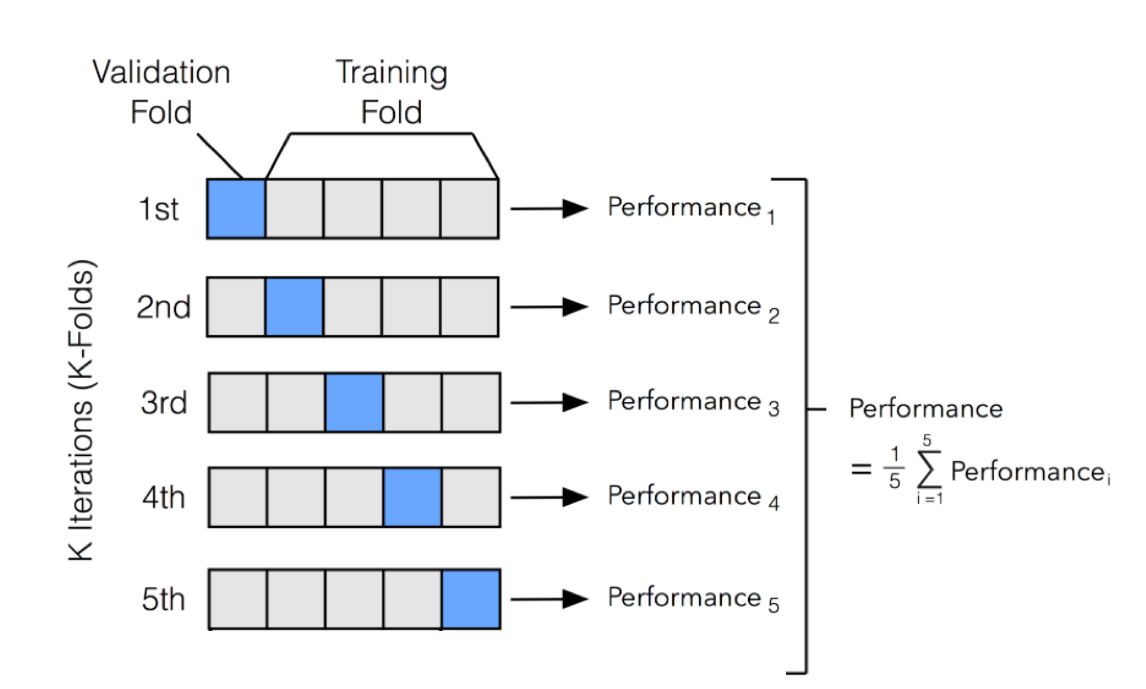
\includegraphics[width = 10cm]{CV-example.png}
		\end{figure}

	\clearpage

	\section{Underfitting vs Overfitting}
		L'overfitting e l'underfitting sono due problemi tipici in cui il modello raggiunge scarse performance nella classificazione dopo l'allenamento ma per motivi diversi.
			\begin{itemize}
				\item $\textbf{Underfitting}:$ ci sono pochi parametri nel modello e un'elevata discrepanza nella classificazione (Alto Bias).
				Il processo di apprendimento è troppo semplice.

				\item $\textbf{Overfitting}:$ ci sono troppi parametri nel modello e un'elevata variabilità della classificazione.
					Il modello è troppo complesso e sensibile ai dati di training (Alta Varianza).
			\end{itemize}

			\begin{figure}[h]
				\caption{Esempio di modello che sottostima}
				\centering
				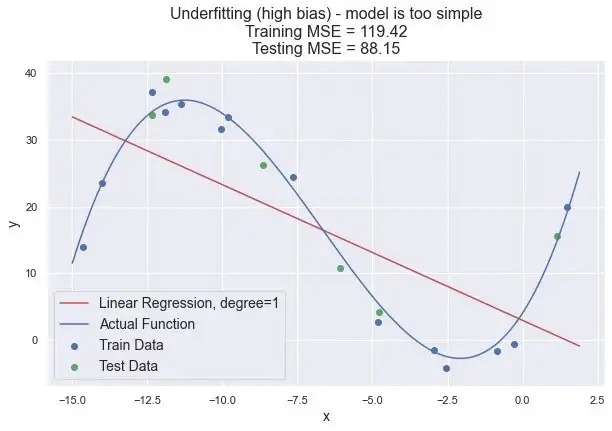
\includegraphics[width = 10cm]{underfitting.png}
			\end{figure}

			\begin{figure}[h]
				\caption{Esempio di modello che sovrastima}
				\centering
				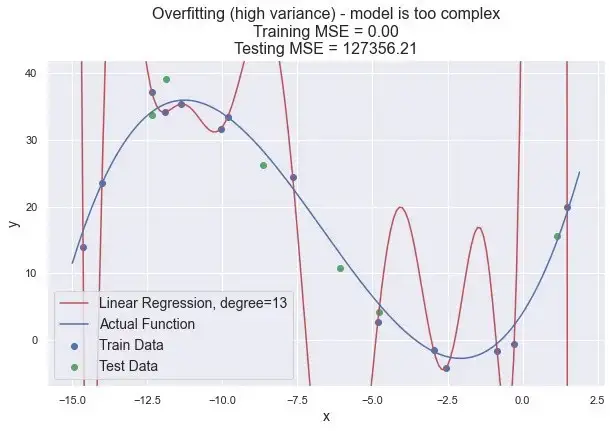
\includegraphics[width = 10cm]{overfitting.png}
			\end{figure}


			\begin{figure}[h]
				\caption{Esempio di modello buono, che non sovrastima o sottostima}
				\centering
				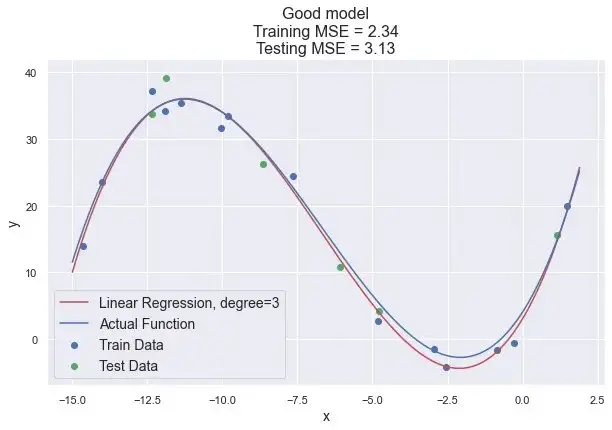
\includegraphics[width = 10cm]{good-model.png}
			\end{figure}

	\clearpage

	\section{ROC: Receiver Operating Characteristics}
		L'analisi delle $\textbf{Receiver Operating Characteristic}$ (ROC) è un approccio grafico per analizzare le prestazioni di un classificatore e studiarne l'output.
		\\[1\baselineskip]
		Utilizza una coppia di statistiche, tasso di Veri Positivi e tasso di Falsi Positivi.
		Le statistiche sono tracciate su un grafico bidimensionale, con tasso di falsi positivi sull'asse delle $x$ e tasso di veri positivi sull'asse delle $y$.
		\\[1\baselineskip]
		Poiché il classificatore può essere un valore arbitrario (output continuo), il confine tra le classi deve essere determinato da un valore di soglia oppure un'etichetta di classe discreta, che indica una delle classi.
		
		\begin{figure}[h]
			\caption[short]{Esempio di grafico ROC}
			\centering
			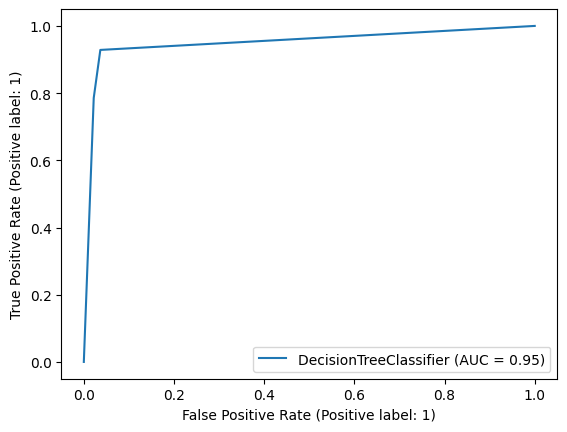
\includegraphics[width = 10cm]{roc-example.png}
		\end{figure}

		\begin{figure}[h]
			\caption[short]{Situazione ideale (1), situazione tipica (2) e situazione peggiore (non risce a discriminare) (3)}
			\centering
			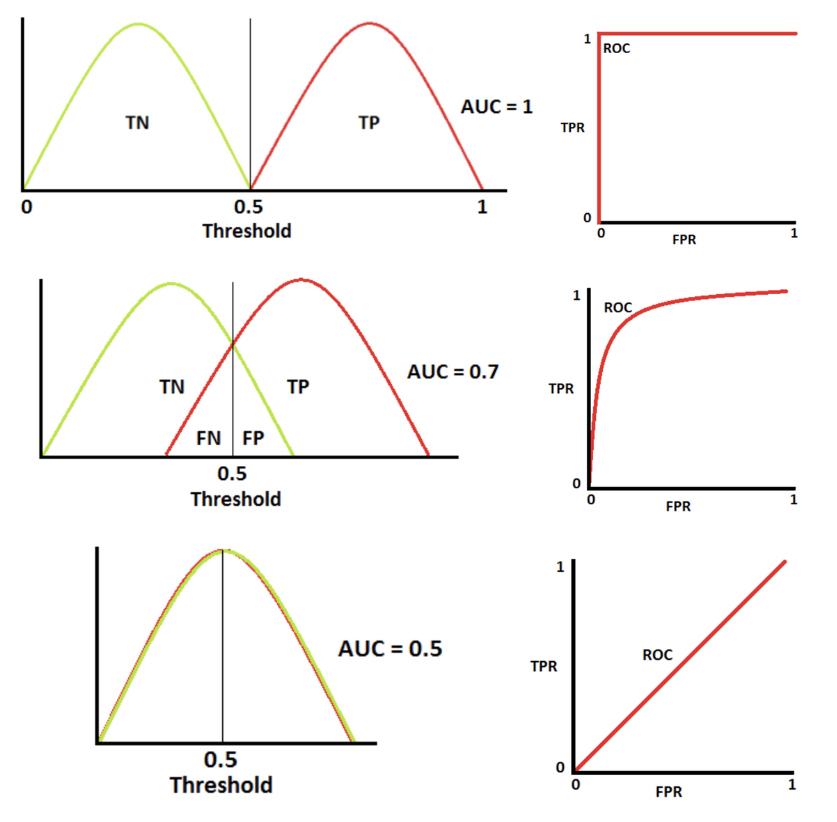
\includegraphics[width = 10cm]{roc-situations.png}
		\end{figure}

	\clearpage
    \chapter{Supervised Learning}

	\section{KNN: K-Nearest-Neighbor}
	L'algoritmo KNN è un classificatore di Supervised Learning che utilizza la vicinanza dei dati per effettuare classificazioni o previsioni sul raggruppamento di un singolo punto.
	Sebbene possa essere utilizzato per problemi di regressione o classificazione, viene generalmente utilizzato come algoritmo di classificazione, basandosi sul presupposto che punti simili possono essere trovati l'uno vicino all'altro.
	\\[1\baselineskip]
	Per problemi di classificazione, un'etichetta di classe viene assegnata sulla base di un voto a maggioranza, ad esempio viene utilizzata l'etichetta più frequentemente rappresentata attorno a un determinato punto.
	I problemi di regressione utilizzano un concetto simile al problema di classificazione, ma in questo caso viene presa la media dei k vicini più vicini per fare una previsione su una classificazione.

	\begin{figure}[h]
		\caption{Esempio di algoritmo kNN}
		\centering
		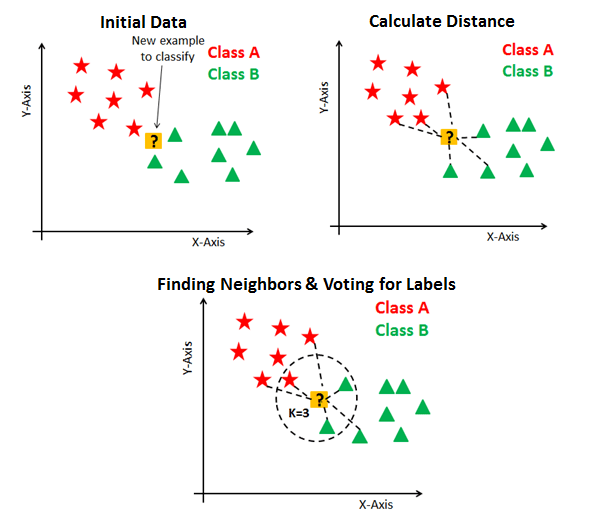
\includegraphics[width = 8cm]{KNN_example.png}
	\end{figure}

		\subsection{Distanza}
			Ovviamente, basandosi sul concetto di vicinanza, bisogna definire la metrica di distanza: la distanza euclidea è una metrica di distanza molto comune, che misura la lunghezza del segmento avente per estremi i due punti.
			$$d(p, q) = \sqrt{(p_{1} - q_{1})^{2} + \dots + (p_{d} - q_{d})^{2}}$$ dove $d$ è la dimensione dello spazio in cui si trovano i punti.
			Per esempio, in uno spazio tridimensionale la formula sarà: $$d(p, q) = \sqrt{(p_{x} - q_{x})^{2} + (p_{y} - q_{y})^{2} + (p_{z} - q_{z})^{2}}$$
			\\[1\baselineskip]
			Bisogna fare attenzione nel caso non si fosse solo interessati a trovare i punti dentro un certo raggio ma si volesse dare più importanza ai punti più vicini a quello preso in questione: un fattore di peso comune è $w = \frac{1}{d^{2}}$.
			\\[1\baselineskip]
			Un altro modo per sensibilizzare la distanza è quello di riscalare i dati. I due metodi più comuni sono:
			\begin{itemize}
				\item $\textbf{StandardScaler}:$ funziona bene se i dati seguono una distribuzione gaussiana/normale. Non rimappa ogni feature nell'intevallo $[0, 1]$ ma dipende dalla variamza: una feature con grande varianza potrebbe impattare fortemente sulla distanza complessiva;
				\item $\textbf{MinMaxScaler}:$ riscala in un range (di default è $[0, 1]$, ma si può modificare). È solitamente più sensibile ai valori anomali, ma pesa le features in maniera più uniforme.
			\end{itemize}

		\subsection{Scelta di K}
			Il valore k nell'algoritmo KNN definisce quanti vicini verranno controllati per determinare la classificazione di un punto specifico.
			Ad esempio, se $k = 1$, l'istanza verrà assegnata alla stessa classe del suo singolo neighbors più vicino.
			\\[2\baselineskip]
			La scelta di $k$ è importante per le performance dell'algoritmo in termini di risultati e di costo computazionale: se $k$ è troppo piccolo l'algoritmo sarà sensibile ai punti di rumore all'interno del dataset, mentre se $k$ è troppo grande il costo di computazione potrebbe crescere di molto.
			\\[1\baselineskip]
			In generale, la scelta di $k$ dipende in gran parte dal dataset poiché i set di dati con più valori anomali probabilmente necessiteranno di valori di $k$ elevati.
			È consigliato di fare tuning del parametro per vedere quale valore porta al risultato migliore e si consiglia di avere un numero dispari per $k$ per evitare pareggi nella classificazione.

		\subsection{Pigrizia e Memoria}
			L'algoritmo KNN fa parte della categoria di algoritmi "lazy", ovvero che il calcolo non viene effettuato durante la sessione di train ma avviene quando viene effettuata una predizione.
			Inoltre fa largo uso della memoria per archiviare i dati di train, il che rende molto costoso in termini di spazio se la dimensionalità dei dati in input è elevata.
\clearpage
	\section{Decision Trees}

    Il $\textbf{Decision Tree Learning}$ è un approccio di apprendimento supervisionato che utilizza un albero decisionale di classificazione o regressione che verrà utilizzato come modello predittivo per trarre conclusioni su un insieme di osservazioni.
    \\[1\baselineskip]
    I modelli ad albero in cui la variabile target può assumere un insieme discreto di valori sono chiamati $\textit{alberi di classificazione}$; in queste strutture ad albero, le foglie rappresentano etichette di classe e i rami rappresentano congiunzioni di caratteristiche che portano a quelle etichette di classe.
    Gli alberi decisionali in cui la variabile target può assumere valori continui (tipicamente numeri reali) sono chiamati $\textit{alberi di regressione}$.
    
    \begin{figure}[h]
        \caption{Esempio di Decision Tree}
        \centering
        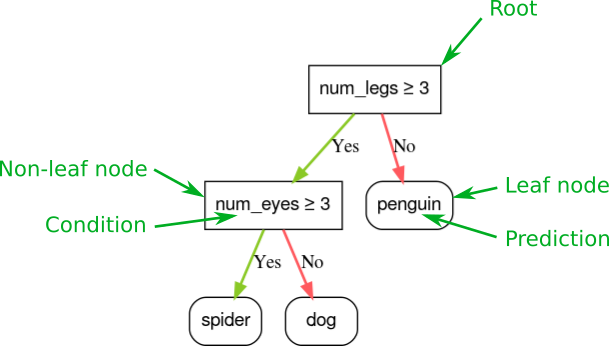
\includegraphics[width = 8cm, height = 4.2cm]{DecisionTree.png}
    \end{figure}

    \subsection{Condizioni Verticali vs Oblique}
        Una condizione verticale (o anche detta "allineata agli assi", "split verticale") coinvolge una sola feature mentre una condizione obliqua coinvolge molteplici features.
        Per esempio, $\textit{num\_legs} \geq 2$ è una condizione verticale mentre $\textit{num\_legs} \geq \textit{num\_eyes}$ è una condizione obliqua.
        \\[1\baselineskip]
        Spesso i Decision Trees sono allenati su condizioni verticali. Tuttavia, lo splitting obliquo è molto più potente perché può esprimere pattern più complessi e può produrre risultati migliori, ad un elevato costo computazionale per il train e l'inferenza.

        \begin{figure}[h]
            \caption{Esempio di Splitting}
            \centering
            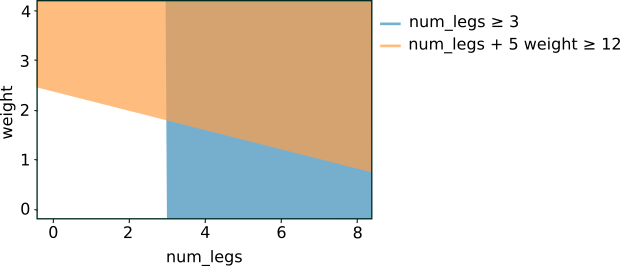
\includegraphics[width = 10cm]{decisiontrees-conditions.png}
        \end{figure}

    \clearpage

    \subsection{Condizioni Binarie vs Non-Binarie}
        Condizioni con due possibili risultati (ad esempio, vero o falso) sono chiamate condizioni binarie.
        Alberi decisionali contenenti solo condizioni binari sono chiamati $\textit{Binary Decision Trees}$.
        \\[1\baselineskip]
        Le condizioni non binarie hanno più di due possibili esiti, dunque hanno un potere discriminante maggiore rispetto a quelle binarie.
        Gli alberi che contengono decisioni una o più condizioni non binarie sono chiamati $\textit{Non-Binary Decision Trees}$.
        \\[1\baselineskip]
        $\textbf{Attenzione}$: Le condizioni non binarie hanno maggiore probabilità di overfit
        
    \subsection{Elenco delle Condizioni più Usate}
        Giusto per essere completi, ecco un elenco dei tipi condizioni che vengono comunemente utilizzate:

        \begin{figure}[h]
            \centering
            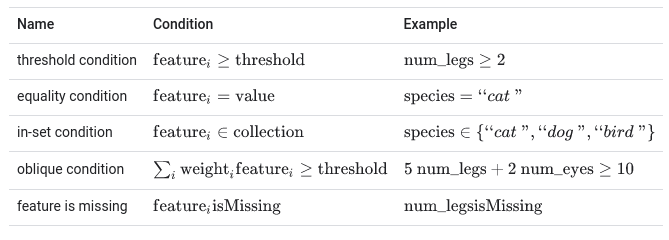
\includegraphics[width = 8.5cm]{conditions-types.png}
        \end{figure}
    
    \clearpage

    \subsection{Costruire un Decision Tree}
        La costruzione del migliore albero decisionale è un problema NP-Hard, dunque viene generalmente utilizzata un'euristica per costruire un albero ottimale.
        La maggior parte degli algoritmi utilizzati per allenare gli alberi decisionali funziona con una strategia greedy in stile $\textit{divide et impera}$: l'algoritmo inizia creando un singolo nodo (la radice) e cresce ricorsivamente, e in maniera greedy, l'albero decisionale.
        Ad ogni nodo, tutte le possibili condizioni vengono valutate e viene assegnato a loro un punteggio; l'algoritmo seleziona la condizione "migliore", ovvero la condizione con il punteggio più alto.\\
        Dopodiché viene eseguito lo split sulla base della condizione precedentemente scelta.
        \\[1\baselineskip]
        L'algoritmo, quindi, ripete ricorsivamente e indipendentemente su tutti i nodi figli, valutando condizioni che non sono ancora state scelte come condizioni di split.
        Quando non vengono trovate condizioni soddisfacenti, il nodo diventa una foglia.
        La predizione nella foglia è scelta come il valore dell'etichetta più significativo.

        \clearpage

        \begin{figure}[h]
            \caption{Esempio di Creazione}
            \centering
            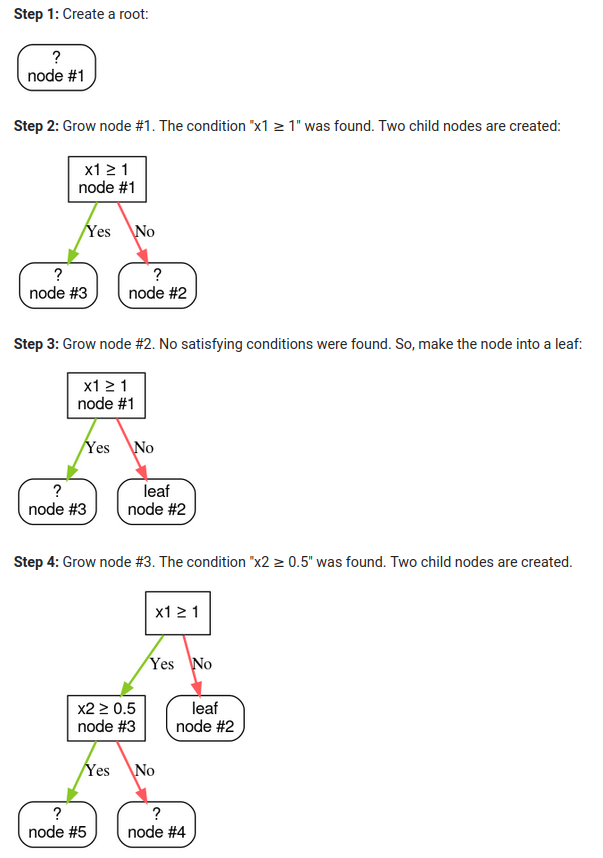
\includegraphics[width = 10cm, height = 12cm]{building-tree-steps.png}
        \end{figure}

        \clearpage

    \subsection{Misura dell'Impurità del Singolo Nodo}
    L'impurità di un nodo misura quanto sono differenti le etichette delle classi per le istanze di dati appartenenti a un nodo comune.
    \\[1\baselineskip]
    Alcune misure che possono essere utilizzate per misurare l'impurità di un certo nodo $t$ sono:

    \begin{itemize}
        \item $\textbf{Entropy}$: $-\sum_{i = 0}^{m-1}{p_{i}(t) \cdot \log_{2}{(p_{i}(t))}}$
            \\[0.5\baselineskip]
            - Massimo: $\log m$, dove $m$ è il numero di classi, quando i records sono equamente distribuiti su tutte le classi, implica poca informazione;
            \\[0.5\baselineskip]
            - Minimo: 0.0 quando tutti i recordi appartengono a una sola classe, implica maggiore informazione (assumiamo che $0 \cdot \log(0) = 0$) (\textbf{"Foglia Pura"}).
            \\
        \item $\textbf{Gini Index}$: $1 - \sum_{i = 0}^{m-1}{p_{i}(t)^{2}}$
            \\[0.5\baselineskip]
            - Massimo: $(1 - \frac{1}{m})$ quando i records sono equamente distribuiti su tutte le classi, implica poca informazione;
            \\[0.5\baselineskip]
            - Minimo: 0.0 quando tutti i records appartengono a una sola classe, implica maggiore informazione.
            \\
        \item $\textbf{Classification Error}$: $1 - \max{[p_{i}(t)]},\ \forall{i}$
            \\[0.5\baselineskip]
            - Massimo: $(1 - \frac{1}{m})$, dove $m$ è il numero di classi, quando i records sono equamente distribuiti su tutte le classi, implica poca informazione;
            \\[0.5\baselineskip]
            - Minimo: 0.0 quando tutti i records appartengono a una classe, implica maggiore informazione.
            \\
        \item $\textbf{Gain Ratio}$: $\frac{\Delta_{\textrm{info}}}{\textrm{SplitInfo}({\cal D})}$ (vedi sotto per $\Delta_{\textrm{info}}$)
            \\[0.5\baselineskip]
            - dove $\textrm{SplitInfo}({\cal D}) = -\sum_{i=0}^{k} {\left[\frac{N(v_{i})}{N} \cdot \log_{2}(\frac{N(v_{i})}{N})\right]}$ con $N(v_{i}) =$ numero di istanze di
                training associate al nodo $v_{i}$ e $N =$ numero di istante di training;
            \\[0.5\baselineskip]
            - Gain Ratio normalizza l'Information Gain per lo SplitInfo di uno split k-ario.
                Per Decision Trees k-ari (invece che binari), l'Information Gain favorisce gli splits con molte piccole partizioni (è più probabile che siano pure);
            \\[0.5\baselineskip]
            - È usato per compensare attributi che producono un gran numero di nodi figlio.
            \\
    \end{itemize}

    dove $p_{i}(t)$ è la frequenza delle istanze di training che appartengono alla classe $i$ al nodo $t$ e $m$ è il numero totale di classi.

    \begin{figure}[h]
        \caption{Cattivo Split vs Buono Split}
        \centering
        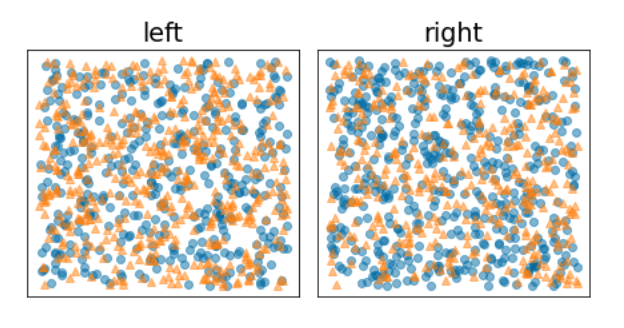
\includegraphics[width = 10cm, height = 6cm]{bad-splitting.png}
        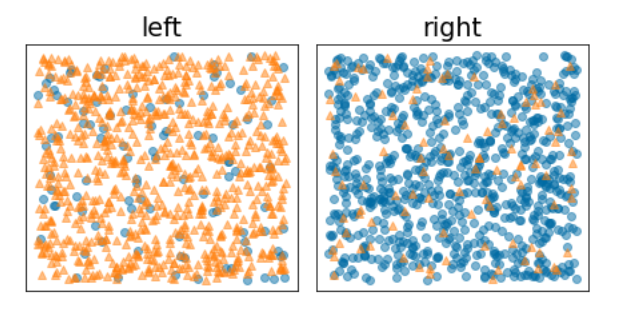
\includegraphics[width = 10cm, height = 6cm]{good-splitting.png}
    \end{figure}

    \clearpage

    \subsection{Impurità Collettiva dei Nodi Figlio}
        Possiamo calcolare l'impurità dei nodi figlio come:
            $$ I(children) = \sum_{i=0}^{k} {\left[\frac{N(v_{i})}{N} \cdot I(v_{i})\right]} $$
        dove:
        \begin{itemize}
            \item $k$ è il numero di nodi figlio;
            \item $N$ è il numero delle istanze di training;
            \item $N(v_{i})$ è il numero di istanze di training associate con il nodo $v_{i}$;
            \item $I(v_{i})$ è l'impurità del nodo $v_{i}$ calcolata con le formule di errore viste prima.
        \end{itemize}

        $\textbf{Esempio:}$ Consideriamo i candidati (a) e (b) per il test della condizione del problema di classificazione dei mutuatari, mostrati nella figura sottostante.
        \begin{figure}[h]
            \centering
            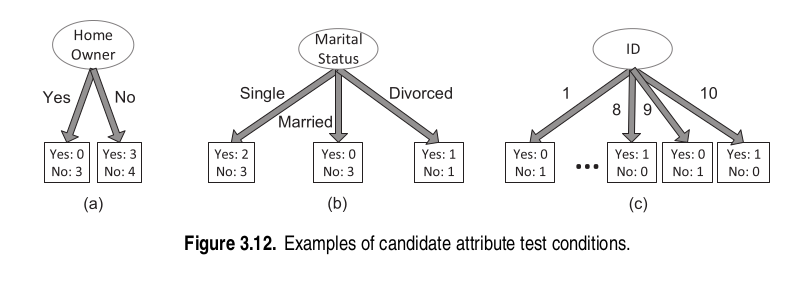
\includegraphics[width = 10cm, height = 3.1cm]{impurity-example.png}
        \end{figure}

        Calcoliamo la $\textbf{Weighted Entropy}$ di Home Owner come segue:
            $$ I(\textrm{Home Owner = Yes}) = - \frac{0}{3} \cdot \log_{2}(\frac{0}{3}) - \frac{3}{3} \cdot \log_{2}(\frac{3}{3}) = 0 $$
            $$ I(\textrm{Home Owner = No}) = - \frac{3}{7} \cdot \log_{2}(\frac{3}{7}) - \frac{4}{7} \cdot \log_{2}(\frac{4}{7}) = 0.985 $$
            $$ I(\textrm{Home Owner}) = \frac{3}{10} \cdot 0 + \frac{7}{10} \cdot 0.985 = 0.690 $$
        \\[1\baselineskip]
        Ora la calcoliamo anche per Marital Status:
            $$ I(\textrm{Marital Status = Single}) = - \frac{2}{5} \cdot \log_{2}(\frac{2}{5}) - \frac{3}{5} \cdot \log_{2}(\frac{3}{5}) = 0.971 $$
            $$ I(\textrm{Marital Status = Married}) = - \frac{0}{3} \cdot \log_{2}(\frac{0}{3}) - \frac{3}{3} \cdot \log_{2}(\frac{3}{3}) = 0 $$
            $$ I(\textrm{Marital Status = Divorced}) = - \frac{1}{2} \cdot \log_{2}(\frac{1}{2}) - \frac{1}{2} \cdot \log_{2}(\frac{1}{2}) = 1.000 $$
            $$ I(\textrm{Marital Status}) = \frac{5}{10} \cdot 0.971 + \frac{3}{10} \cdot 0 + \frac{2}{10} \cdot 1.0 = 0.686 $$
            \\[1\baselineskip]
        Come possiamo vedere, l'impurità di Marital Status è leggermente più alta rispetto a Home Owner.

        \clearpage

        \subsection{Trovare la migliore condizione per il test degli attributi}
            Per determinare la bontà di una condizione di test, dobbiamo confrontare il grado di impurità del nodo genitore (prima della divisione) con il grado pesato di impurità dei nodi figli (dopo la divisione).
            \\
            Maggiore è la loro differenza, migliore è la condizione del test. Questa differenza, $\Delta$, definita anche come il guadagno ($\textbf{Gain}$) in purezza di una condizione di test, può essere definita come segue:
                $$ \Delta = I(\textrm{parent}) - I(\textrm{children}) $$

            Maggiore è il guadagno, più pure sono le classi nei nodi figli rispetto al nodo genitore. Il criterio di suddivisione nell'algoritmo di Decision Tree seleziona la condizione di test che mostra il guadagno massimo.
            \\[1\baselineskip]
            Infine, quando l'entropia è usata come misura di impurità, la differenza di entropia tra genitore e figli è comunemente nota come $\textbf{Information Gain}$, $\Delta_{\text{info}}$.

            \begin{figure}[h]
                \centering
                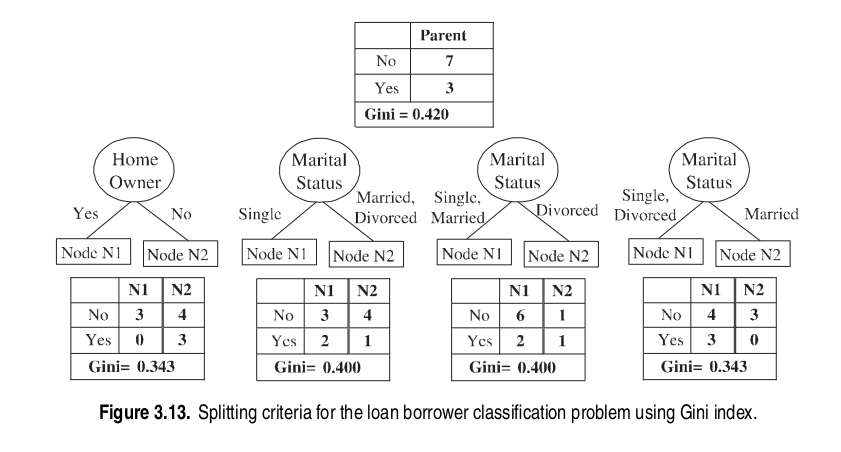
\includegraphics[width = 10cm, height = 6.5cm]{best-attribute-example.png}
            \end{figure}

            \clearpage

	\section{Logistic Regression}
    La $\textbf{Logistic Regression}$ è una funzione definita come $$ sig(t) = \frac{1}{1+e^{-t}} $$
    e stima la probabilità che si verifichi un certo evento sulla base di un determinato set di dati di variabili indipendenti.
    
    \begin{figure}[h]
        \caption{Regressione Lineare vs Regressione Logistica}
        \centering
        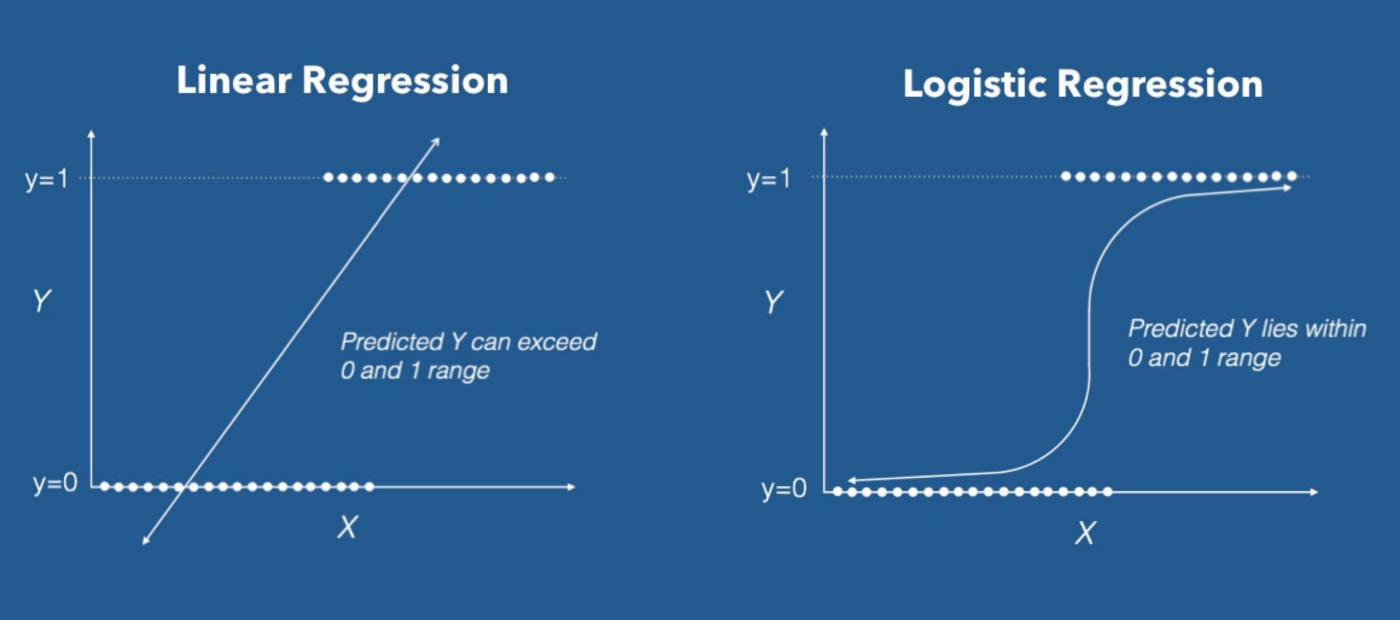
\includegraphics[width = 10cm]{logistic-regression-example.jpeg}
    \end{figure}
    
    \clearpage

    Questo classificatore calcola la retta che separa una classe dall'altra, in uno spazio a due o più dimensioni.
    Tra le infinite rette che possono dividere due classi viene scelta, generalmente, quella che le divide a distanza equa dalla retta.
    È possibile, però, scegliere una retta diversa nel caso si voglia essere più restrittivi verso una classe rispetto a un'altra.
    \\[1\baselineskip]
    $\textbf{NOTA:}$ Poiché il risultato è una probabilità, la variabile dipendente ($Y$) è limitata nell'intervallo $[0,1]$.

    \clearpage
	\section{SVM: Support Vector Machine}
    La $\textbf{SVM}$ è un modello di Supervised Learning che utilizza algoritmi di classificazione per problemi di classificazione tra due gruppi.
    \\[1\baselineskip]
    Rispetto agli algoritmi più recenti (come le reti neurali), presenta due vantaggi principali: maggiore velocità e migliori prestazioni con un numero piccolo di campioni.
    
    \begin{figure}[h]
        \caption{Esempio di SVM}
        \centering
        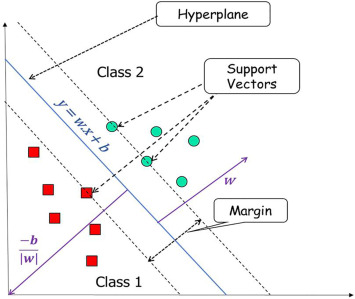
\includegraphics[width = 10cm, height = 6.7cm]{SVM-example.jpg}
    \end{figure}
    
    \clearpage

    Una SVM prende i punti del dataset e calcola l'iperpiano che separa meglio i due gruppi.
    \\
    Questa linea è la $\textbf{Decision Boundary}$ (nell'esempio sopra, tutto ciò che cade da un lato sarà classificato come rosso mentre tutto ciò che cade nell'altro sarà verde).
    \\[1\baselineskip]
    Per la SVM, il miglior iperpiano è quello che massimizza i margini dei vettori di support di ciascuna classe.
    In altre parole, trova l'iperpiano la cui distanza dell'elemento più vicino (possono essere anche più di uno se sono equamente vicini all'iperpiano) di ciascuna classe è la più grande.

    \subsection{Margini}
        Il $\textbf{margine}$ è la distanza che abbiamo tra i punti più vicini al nostro Decision Boundary, ovvero la retta.
        \\
        Esistono due tipi di margini:
        \begin{itemize}
            \item $\textbf{Hard Margin}:$ è il margine che possiamo usare quando riusciamo a separare tutti i punti da una parte e dall'altra, senza mischiarli;
            \item $\textbf{Soft Margin}:$ rilassa i vincoli dell'hard margin, permettendo che alcuni punti che dovrebbero appartenere a una classe di "sorpassare" la retta.
                Questo permette di avere meno restrizioni nel caso non esista una retta che separe bene i due cluster.
        \end{itemize}

    \subsection{Problemi di separazione non lineare}
        Immaginiamo di avere un problema del genere:

        \begin{figure}[h]
            \caption{Esempio di problema non lineare}
            \centering
            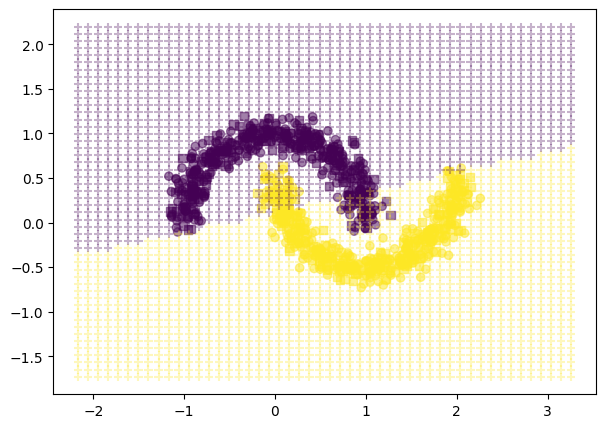
\includegraphics[width = 10cm, height = 6cm]{non-linear-problem.png}
        \end{figure}

        Per questo problema non esiste un iperpiano di due dimensioni che separa i due cluster di dati.
        \\
        La soluzione a tale problema è quella di aumentare la dimensione dello spazio su cui si sta lavorando per vedere se esiste un iperpiano che separa i due clusters.
        Dopo aver trasformato lo spazio, si può usare il regressore nel nuovo spazio creato.

        \begin{figure}[h]
            \caption{Aumento di una dimensione dello spazio}
            \centering
            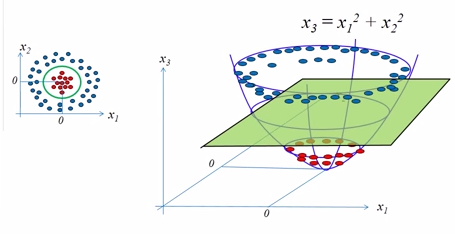
\includegraphics[width = 10cm, height = 4cm]{esempio-spazio.png}
        \end{figure}

        \begin{figure}[h]
            \caption{Risultato del regressore nel nuovo spazio}
            \centering
            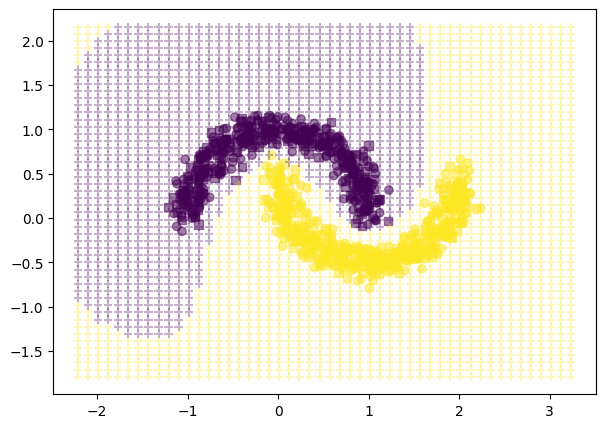
\includegraphics[width = 10cm, height = 5cm]{risoluzione-problema.png}
        \end{figure}

    \clearpage
	\section{Linear Regression}
    La $\textbf{Regressione Lineare}$ è un modello molto semplice basato sull'equazione della retta e viene utilizzata per studiare la relazione tra due o più variabili.
    \\[1\baselineskip]
    Nella Regressione Lineare viene utilizzato tipicamente l'errore quadratico medio (MSE):
        $$ \textrm{MSE} = \frac{1}{n} \sum_{i=0}^{n}{\left( y_{i} - \hat{y_{i}} \right)^2} $$
    dove $n$ è la dimensione del campione, $y_{i}$ sono le osservazioni e $\hat{y_{i}}$ sono i valori stimati dal modello.
    \\[1\baselineskip]
    Il MSE è una misura di qualità del modello: più bassa è, migliore sarà il nostro modello!
    \\[1\baselineskip]
    La Regressione Lineare si divide in $\textit{semplice}$ quando viene stiamo un modello della forma $y = \beta_{0} + \beta_{1} x$ e
    $\textit{multipla}$ quando stimiamo un modello che utilizza più di un predittore, per esempio $y = \beta_{0} + \beta_{1} \log(x) + \beta_{2} x^{2}$.

    \clearpage
    \chapter{Ensemble Methods}

    \section{Introduzione}
    $\textbf{L'analisi dei Clusters}$ si pone l'obiettivo di trovare le similarità tra i dati secondo le caratteristiche trovate nei dati stessi e raggruppare i dati simili tra loro in $\textbf{clusters}$, ovvero delle collezioni di dati.
    \\[1\baselineskip]
    Questo tipo di problemi fanno parte della seconda famiglia di apprendimento, ovvero $\textbf{Unsupervised Learning}$: non ci sono etichette di classe già predefinite, ma l'algoritmo deve imparare da solo attraverso l'osservazione e l'analisi dei dati.
    \\[1\baselineskip]
    Il risultato di un'ottima procedura di clustering prevede come risultato dei clusters che hanno:
        \begin{itemize}
            \item $\textbf{Alta Similarità "Intra-Class"}:$ ogni dato è molto simile a tutti gli altri dati del cluster;
            \item $\textbf{Bassa Similarità "Inter-Classe"}:$ ogni dato è molto dissimile da tutti gli altri dati fuori dal cluster.
                \\[1\baselineskip]
        \end{itemize}

    Tra i vari approcci per la risoluzione dei problemi di clustering, i tre più comuni sono:
        \begin{itemize}
            \item $\textbf{Partitioning}:$ vengono costruite varie partizioni e valutate secondo alcuni criteri (es: minimizzazione del Sum of Square Errors);
            \item $\textbf{Hierarchical}:$ viene creata una decomposizione gerarchica del dataset usando alcuni criteri;
            \item $\textbf{Density-Based}:$ approccio basato su funzioni di densità e connettività.
        \end{itemize}

\clearpage
    \section{Bagging vs Boosting}
    \subsection{Bagging}
        Il BAGGing (Boostrap AGGregation) è un Ensemble Method utilizzato per ridurre la varianza all'interno di un dataset con molto rumore.
        \\[1\baselineskip]
        Nel Bagging, un campione casuale di dati di training viene selezionato con il metodo della sostituzione, ovvero che all'interno di quel campione casuale è possibile selezionare lo stesso dato più di una volta (la probabilità è uniforme).
        Dopo aver generato diversi campioni, questi Weak Learners vengono allenati parallelamente e indipendentemente l'uno dall'altro per poi utilizzare, a seconda del problema, una media o il voto di maggioranza come stima.

    \subsection{Boosting}
        Il Boosting è un Ensemble Method utilizzato per ridurre al minimo gli errori durante la fase di training.
        \\[1\baselineskip]
        Nel Boosting, un campione casuale di dati di training viene selezionato con ripetizione (come nel bagging) e utilizzato per addestrare in sequenza ogni modello: ogni modello cerca di compensare i punti deboli del proprio predecessore.
        I pesi dei dati vengono ripesati: i dati classificati in modo errato ottengono un peso maggiore mentre quelli classificati correttamente perdono peso. Pertanto, i Weak Learners successivi si concentreranno maggiormente sui dati che i precedenti hanno classificato erroneamente.
        \\[1\baselineskip]
        La ricalibrazione del peso di ogni dato indica una ricalibrazione della probabilità con la quale quel dato può essere pescato come campione dal modello successivo: più è alta e più probabilità avrà di essere scelto (solo all'inizio i pesi sono tutti uniformi),

    \subsection{Differenze}
        Le principali differenze tra questi due metodi sono:
        
        \begin{itemize}
            \item Il modo in cui vengono allenati: nel bagging, i Weak Learners vengono addestrati in parallelo mentre nel boosting imparano in sequenza;
            \item Il campionamento dei dati per la fase di addestramento: il bagging prende i dati con la stessa probabilità mentre il boosting li prende in base al peso dato dai modelli precedenti;
            \item Gli scenari in cui vengono utilizzati: il Bagging funziona bene per Weak Learners con alta varianza e bassa distorsione, mentre il Boosting quando si osserva una bassa varianza e un'elevata distorsione.
        \end{itemize}

    \clearpage
    \section{Random Forest}
    $\textbf{Random Forest}$ (o $\textbf{Random Decision Forest}$) è un Ensemble Method per la classificazione, la regressione e altre attività (es: Stima di Similarità o Feature Selection).
    Opera costruendo una moltitudine di alberi decisionali durante la fase di training, seguendo l'idea degli algoritmi di Bagging.
    L'output della foresta dipende dal tipo di attività: se di classificazione sarà la classe selezionata dalla maggioranza degli alberi, se di regressione sarà la predizione media degli alberi.
    \\[1\baselineskip]
    Le Random Forest correggono l'abitudine degli albero decisionali di adattarsi in modo eccessivo ($\textbf{overfitting}$) al loro set di allenamento.
    \\[1\baselineskip]
    In particolare, gli alberi che crescono molto in profondità tendono ad apprendere schemi molto irregolari: fanno overfitting sul loro train set, cioè hanno una bassa distorsione ma una varianza molto alta.
    Le Random Forest sono un modo per utilizzare le predizioni di più alberi decisionali, addestrati su parti diverse dello stesso train set, con l'obiettivo di ridurre la varianza.
    \\
    Ciò avviene a scapito di un piccolo aumento della distorsione e una certa perdita di interpretabilità, ma, generalmente, aumenta notevolemte le prestazioni del modello finale.

    \subsection{R.F. come Stimatore di Similarità}
        In definitiva, $\underline{\textrm{un modello raggruppa istanze simili}}$ e fornisce la stessa previsione per esse.
        \\[1\baselineskip]
        Un albero decisionale utilizza i predicati dei nodi per identificare un sottoinsieme di istanze per le quali viene fornita la stessa previsione: questo raggruppamento per somiglianza si basa sull'etichetta target piuttosto che sulle features.
        \\
        In un certo senso, questo supera il problema di pesare correttamente le caratteristiche per calcolare la somiglianza: quali caratteristiche sono rilevanti e come determinare se due istanze sono simili è implicitamente determinato dall'algoritmo di allenamento.
        \\[1\baselineskip]
        Possiamo costruire una misura di similarità sulla base della seguente ipotesi: due istanze sono simili se attraversano la foresta casuale lungo percorsi simili, ovvero se cadono sulle stesse foglie.
        
        Misuriamo quindi la somiglianza tra due istanze ($o_{i}$ e $o_{j}$) come il rapporto tra il numero di foglie comuni raggiunte durante l'attraversamento della foresta e il numero di alberi ($n$) in cui i due dati appaiono nella stessa foglia:

            $$ RF_{sim}(o_{i}, o_{j}) = \frac{1}{n} \cdot \sum_{k=0}^{n}{\left[ \textrm{leaf}_{k}(o_{i}) == \textrm{leaf}_{k}(o_{j}) \right]} $$

        In linea di principio, questo potrebbe essere applicato a qualsiasi foresta di alberi decisionali, inclusi il bagging e il boosting.
        \\
        Random Forest è preferibile per i seguenti motivi:
        \begin{itemize}
            \item La R.F. è migliore del Boosting poiché la R.F. dà lo stesso peso agli alberi;
            \item La R.F. è migliore di Bagging in quanto i suoi alberi sono più diversi.
        \end{itemize}

    \subsection{Identificare gli Outliers con le R.F.}
        Con un ragionamento simile al concetto di similarità, possiamo usare le Random Forest per identificare gli outliers nel dataset.
        \\
        Definiamo l'$\textbf{Outlying Score}$ come l'inverso della somma dei quadrati delle similarità tra il nodo $o_{i}$ preso in questione e ogni altro nodo nel dataset:

            $$ out(o_{i}) = \left[ \sum_{o_{j} \in \cal{D}}{RF_{sim}(o_{i}, o_{j})^{2}} \right]^{-1}; \qquad \forall{o_{j} \neq o_{i}} $$
    
    \subsection{Feature Importance \& Feature Selection}
        $\textbf{Importanza:}$ ogni albero della foresta può calcolare l'importanza di una feature in base alla capacità della feature stessa di aumentare la purezza delle foglie.
        \\
        Maggiore è l'incremento della purezza delle foglie, maggiore è l'importanza della caratteristica. Questo viene fatto per ogni albero, quindi viene calcolata la media tra tutti gli alberi e, infine, normalizzata nell'intervallo $[0,1]$.
        \\[2\baselineskip]
        $\textbf{Selezione:}$ Una volta individuata l'importanza di ogni feature, esegue la selezione delle features utilizzando una procedura chiamata $\textbf{R.F.E}$ (Recursive Feature Elimination).
        È comune combinare questa tecnica con la Cross-Validation.
        \\[1\baselineskip]
        L'idea è quella di rimuovere la feature meno rilevate dopo il fitting del modello, calcolare le performance usando la [k-fold] Cross-Validatio.
        Questa sequenza di operazioni vengono iterate fino all'esaurimento di tutte le features.
        Il set di features con il più alto punteggio di performance calcolato durante tutto il procedimento è il set di features ritenuto migliore dalla R.F.
        
    \clearpage
    \section{Naive Bayes}
    $\textbf{Naive Bayes}$ è una tecnica semplice per costruire classificatori.
    Non esiste un unico algoritmo per addestrare tali classificatori, ma una famiglia di algoritmi basati su un principio comune: tutti i classificatori $\textit{ingenui}$ (naive) presuppongono che
    il valore di una particolare feature sia $\textbf{indipendente}$ dal valore di qualsiasi altra feature.
    \\[1\baselineskip]
    Prende il nome di Naive Bayes dal $\textbf{Teorema di Bayes}$:
        $$ P \left[ X\ |\ Y \right] = \frac{P \left[ Y\ |\ X \right] \cdot P \left[ X \right]}{P \left[ Y \right]} $$
    
    da cui si può implicare che:
        $$ P \left[ Y\ |\ X \right] \cdot P \left[ X \right] = P \left[ X\ |\ Y \right] \cdot P \left[ Y \right] = P \left[ X,\ Y \right] $$
    \\[1\baselineskip]
    In Machine Learning, il problema si traduce in trovare $P \left[ y\ |\ X \right]$ o, nel caso di molteplici classi $C_{1}, \dots, C_{m}$, trovare
        $$ \arg \max_{C_i} \left[ P \left( C_{i}\ |\ X \right) \right] $$

    Assumendo che ogni feature è condizionalmente indipendente dalle altre:
        $$ P(C_i |X) = P(x_1 | C_i) \cdot P(x_2 | C_i) \cdot \ldots P(x_f | C_i) $$
    
    la predizione del modello sarà:
        $$ \arg \max_{C_i} \left[ P \left( C_{i}\ |\ X \right) \right] = P(x_1 | C_i) \cdot P(x_2 | C_i) \cdot \ldots P(x_f | C_i) \cdot \frac{P(C_i)}{P(X)} $$

    Siccome $P \left( X \right)$ non cambia il ranking delle classi $C_{i}$ possiamo anche rimuoverlo dall'equazione, se per scopi di classificazione:
        $$ \arg \max_{C_i} \left[ P \left( C_{i}\ |\ X \right) \right] = P(x_1 | C_i) \cdot P(x_2 | C_i) \cdot \ldots P(x_f | C_i) \cdot P(C_i) $$

    \clearpage

    \begin{figure}[h]
        \caption[short]{Esempio di classificazione}
        \centering
        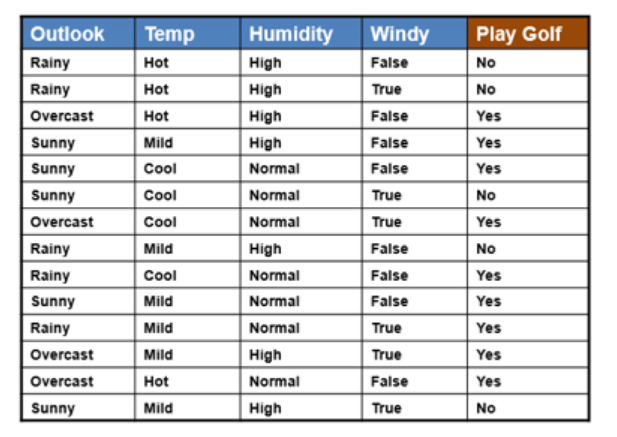
\includegraphics[width = 10cm]{table-bayes-example1.png}
        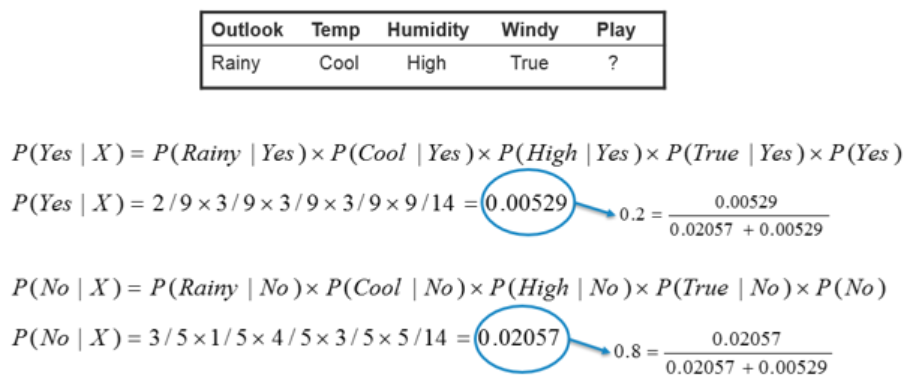
\includegraphics[width = 10cm]{table-bayes-example2.png}
    \end{figure}

    \clearpage

    \subsection{Zero-Frequency Problem}
        Nel caso una certa probabilità $P \left( x_{j}\ |\ C_{i} \right) = 0$, l'intero prodotto andrebbe anch'esso a zero, pure se i segnali delle altre features sono molto forti!
        \\
        Per ovviare a questo problema si utilizza la $\textbf{Correzione di Laplace}$
            $$ P(x_{j}\ |\ C_{i}) = \frac{N_{ij} + 1}{N_{i} + v} $$

        dove:
            \begin{itemize}
                \item $N_{ij}$ è il numero di istanze in classe $C_{i}$ con la $j$-esima feature uguale a $x_{j}$;
                \item $N_{i}$ è il numero di istanze in classe $C_{i}$;
                \item $v$ è il numero totale di valori unici della $j$-esima feature nel dataset $\cal D$.
            \end{itemize}

        $\textbf{Nota:}$ questa correzione deve essere applicata a ogni feature ordinale e non solo a quella per cui accade il problema della frequenza a zero!

    \clearpage
    \chapter{Feature Engineering}
    Durante il corso della creazione di un modello, è molto probabile (quasi certo) di incontrare problemi con i dati.
    Alcune problematiche che potrebbero sorgere sono, per esempio, la gestione delle features binarie, gestione delle features categoriali o anche dei valori mancanti!
    \\[2\baselineskip]
    Di seguito verranno illustrate alcune strategie per ovviare a questi problemi:
    \begin{itemize}
        \item $\textbf{Features Categoriche Binarie}:$ fare un remapping a 0-1 dei valori (es: Alto $\longrightarrow$ 1; Basso $\longrightarrow$ 0);
        \item $\textbf{Features Categoriche K-arie}:$ One-Hot Encoding (discusso in seguito);
        \item $\textbf{Etichette di Classe Categoriche K-arie}:$ fare un remapping a degli ID numerici;
            \\
            $\textbf{Attebzione:}$ Questa soluzione va bene per i Decision Trees ma non per kNN e Linear Regression!
        \item $\textbf{Features con Valori Singoli}:$ essendo insignificative alla risoluzione di qualsiasi tipo di problema, le si può tranquillamente togliere;
        \item $\textbf{Valori Mancanti}:$ rimpiazzare con la media se è un valore numerico o con la moda se categoriale.
    \end{itemize}

    \subsection{Problemi con i Dati Categoriali}
        Alcuni algoritmi possono funzionare direttamente con i dati categoriali (es: Alberi Decisionali), ma molti altri algoritmi non riescono a processarle e richiedono una trasformazione numerica di queste variabili.

        \subsubsection{Codifica a Numerici Ordinali}
            A ogni valori categorico viene assegnato un valori intero (es: "rosso" $\longrightarrow$ 1, "verde" $\longrightarrow$ 2, "blu" $\longrightarrow$ 3).
            \\[1\baselineskip]
            Bisogna fare attenzione nell'utilizzo di questo metodo perché si va a creare una relazione di ordinamento.
            Questo può essere d'aiuto se si vuole effettivamente rappresentare un ordinamente, ma nelle variabili categoriali in cui non esiste una relazione d'ordine ciò può portare a risultati imprevisti!
            \\
            Prendiamo d'esempio la codifica in valori ordinali del colore degli occhi: dire che "rosso" (1) è tre volte più piccolo di "blu" (3) non ha senso in questo caso.

        \subsubsection{One-Hot Encoding}
            Questo metodo di codifica consiste nella sostituzione della variabile categoriale con $n$ variabili binarie, una per ogni valore che poteva assumere la precedente feature categoriale.
            \begin{figure}[h]
                \caption[short]{Esempio di One-Hot Encoding}
                \centering
                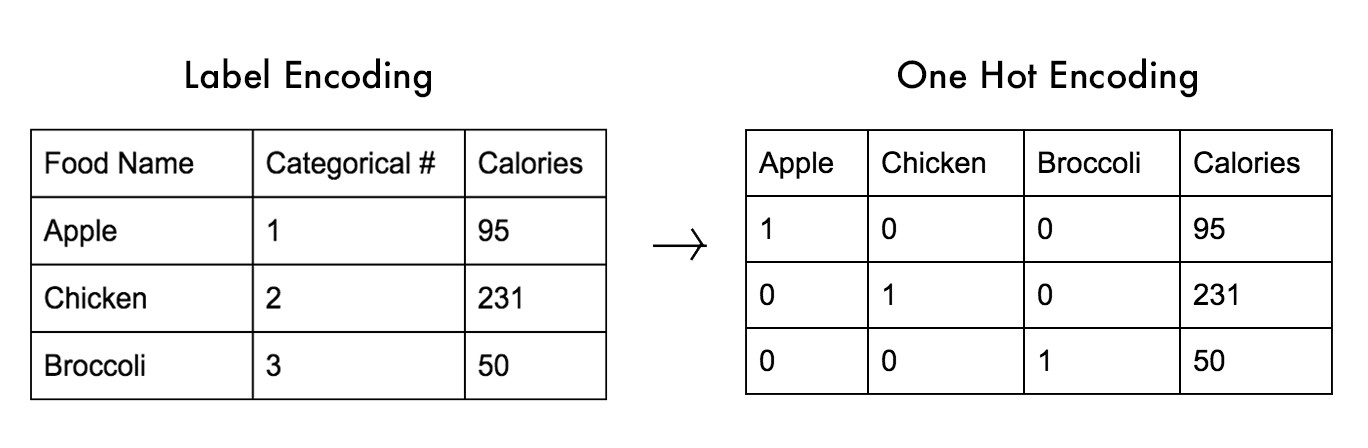
\includegraphics[width = 10cm, height = 2.3cm]{one-hot-example.jpeg}
            \end{figure}
        
    \clearpage
    \chapter{Text Processing}
    Di seguito alcuni metodi per processare dei testi:

    \begin{itemize}
        \item $\textbf{TF-IDF}$ (Term Frequency - Inverse Document Frequency): è un algoritmo che utilizza la frequenza delle parole per determinare quanto tali parole siano rilevanti per un dato documento.
        \\
        È un approccio relativamente semplice ma intuitivo per dare peso alle parole.
        \\[1\baselineskip]
        Per riassumere l'intuizione chiave, l'importanza di un termine è inversamente correlata alla sua frequenza nei documenti.
        \\[1\baselineskip]
        TF ci fornisce informazioni sulla frequenza con cui un termine $t$ appare in un documento $d$ e IDF ci fornisce informazioni sulla relativa rarità di un termine $t$ nella raccolta dei documenti $D$.
        Moltiplicando questi valori insieme possiamo ottenere il nostro valore TF-IDF finale.

            $$ tf\ idf(t, d, D) = tf(t, d) \cdot idf(t, D) $$

        dove $idf(t, D)$ è definito come:
            $$ idf(t, D) = \ln \left( \frac{N_{\textrm{docs}}}{df(t)} \right)$$
        
        in cui $N_{\textrm{docs}}$ rappresenta il numero di documenti nella collezione $D$ mentre $df(t)$ è il numero di documenti contenenti il termine $t$;
        \\[0.5\baselineskip]

        \item $\textbf{Stemming}:$ viene usato per rimuovere il prefisso/suffisso (es: "being" $\longrightarrow$ "be", "was" $\longrightarrow$ "was");
            \\[0.5\baselineskip]
        \item $\textbf{Lemming}:$ si riferisce all'identificazione dell'origine della parola (es: "being" $\longrightarrow$ "be", "was" $\longrightarrow$ "be").
    \end{itemize}

    \clearpage
    \chapter{Dimensionality Reduction}
    \section{Curse of Dimensionality}
        La Maledizione della Dimensionalità ($\textbf{Curse of Dimensionality}$) si riferisce a una serie di problemi che sorgono quando si lavora con dati ad alta dimensione.
        \\[1\baselineskip]
        La dimensione di un set di dati corrisponde al numero di attributi/features che esistono in un set di dati.
        Un set di dati con un numero elevato di attributi, generalmente dell'ordine di un centinaio o più, viene definito dati ad alta dimensione.
        \\[1\baselineskip]
        Alcune delle difficoltà che derivano dai dati ad alta dimensione si manifestano durante l'analisi o la visualizzazione dei dati per identificare i modelli, e alcune si manifestano durante l'allenamento dei modelli stessi.
        \\[1\baselineskip]
        All'aumentare della dimensionalità, il numero di punti richiesti per una buona prestazione di qualsiasi algoritmo aumenta in modo esponenziale.
        Il motivo è che avremmo bisogno di un numero sempre più grande di punti per una data combinazione di features, affinché qualsiasi modello di apprendimento sia valido.

        \begin{figure}[h]
            \caption{Relazione tra Performance e Dimensionalità}
            \centering
            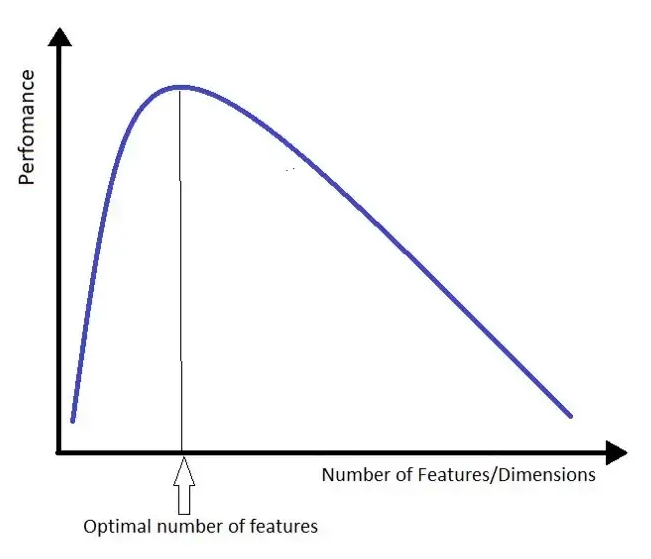
\includegraphics[width = 10cm]{dimensionality-curse-curve.png}
        \end{figure}

    \clearpage

    \section{PCA: Principal Component Analysis}
        L'analisi delle componenti principali, o $\textbf{PCA}$, è un metodo per la riduzione della dimensionalità che viene spesso utilizzato per ridurre la dimensionalità di set di dati di grandi dimensioni, trasformando un set di variabili di grandi dimensioni in uno più piccolo che contiene ancora la maggior parte delle informazioni nel set di dati originale.
        \\[1\baselineskip]
        La riduzione del numero di variabili di un set di dati va naturalmente a scapito dell'accuratezza, ma il trucco nella riduzione della dimensionalità è scambiare un po' di accuratezza con la semplicità: proprio perché i set di dati più piccoli sono più facili da esplorare e visualizzare, rendono l'analisi dei dati molto più semplice e veloce per gli algoritmi.
        \\[1\baselineskip]
        Quindi, per riassumere, l'idea di PCA è semplice: ridurre il numero di variabili di un set di dati, preservando quante più informazioni possibili.

        \subsection{Funzionamento}
            $\textbf{Nota:}$ non sono state elencate tutte a lezione, ma vengono lo stesso inserite (per completezza).
            \\[1\baselineskip]
            La PCA può essere suddivisa in cinque steps:

            \begin{enumerate}
                \item Standardizzare l'intervallo di variabili continue;
                \item Calcolare la matrice di covarianza/correlazione per identificare le correlazioni;
                \item Calcolare gli autovettori e gli autovalori della matrice di covarianza per identificare le componenti principali;
                \item Crea un vettore di caratteristiche per decidere quali componenti principali mantenere;
                \item Esegue un recasting dei dati lungo gli assi delle componenti principali.
            \end{enumerate}
        
            PCA trova le direzioni ortogonali della varianza massima dei dati forniti.
            Può essere pensato come una trasformazione in un nuovo sistema di coordinate, dove la prima coordinata (la prima componente principale) identifica la proiezione di massima varianza, la seconda coordinata la seconda massima varianza, etc...
            \\[1\baselineskip]
            Matematicamente, i componenti principali sono gli autovettori della matrice di covarianza.

            \begin{figure}[h]
                \caption[short]{Esempio di PCA}
                \centering
                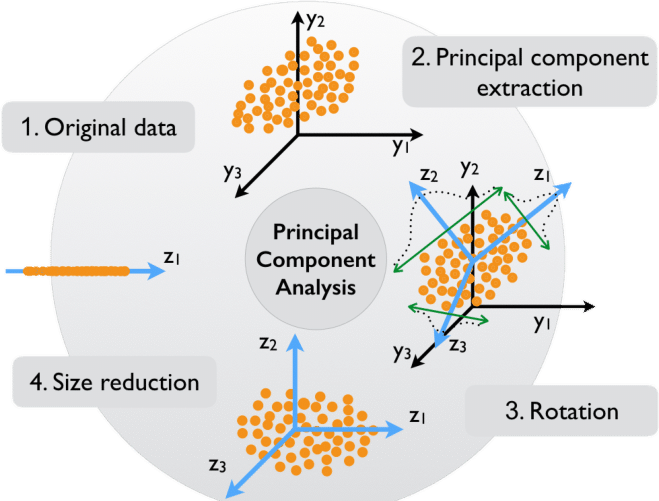
\includegraphics[width = 10cm]{PCA-example.png}
            \end{figure}
        
        \clearpage

        \subsection{Come trova le Componenti Principali?}
            Poiché ci sono tante componenti principali quante sono le variabili nei dati, le componenti principali sono costruite in modo tale che la prima componente principale rappresenti la massima varianza possibile nel set di dati.
            \\[1\baselineskip]
            $\textbf{Nota:}$ oltre alla massimizzazione della varianza (nell'esempio sottostante, la distanza fra i punti blu), si cerca anche di minimizzare la perdita di informazione (distanza tra la componente e i punti arancioni).
            
            \begin{figure}[h]
                \centering
                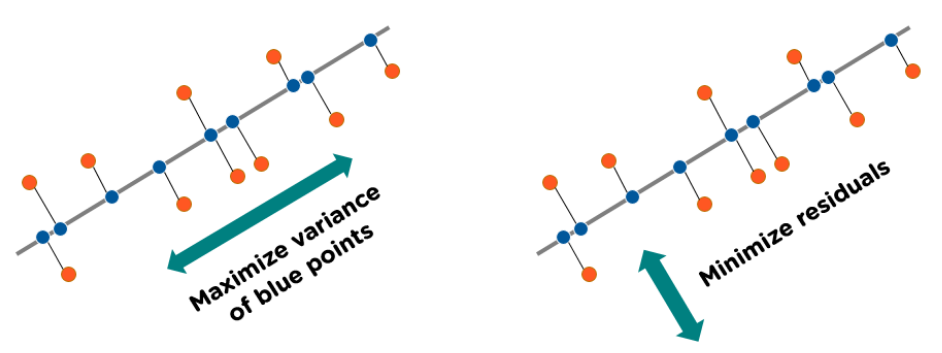
\includegraphics[width = 10cm]{PCA-example2.png}
            \end{figure}
            
            La seconda componente principale viene calcolata allo stesso modo, con la condizione che sia incorrelata con (cioè perpendicolare a) la prima componente principale e che tenga conto della successiva varianza più alta.
            Questo continua fino a quando non è stato calcolato un totale di $d$ componenti principali, pari al numero originale di variabili.
            \\[1\baselineskip]
            Alla fine del procedimento, i primi $m$ componenti con $m \le d$ ($d$ è la dimensione iniziale del dataset) diventeranno le nuove dimensioni del nuovo set di dati.

            \begin{figure}[h]
                \centering
                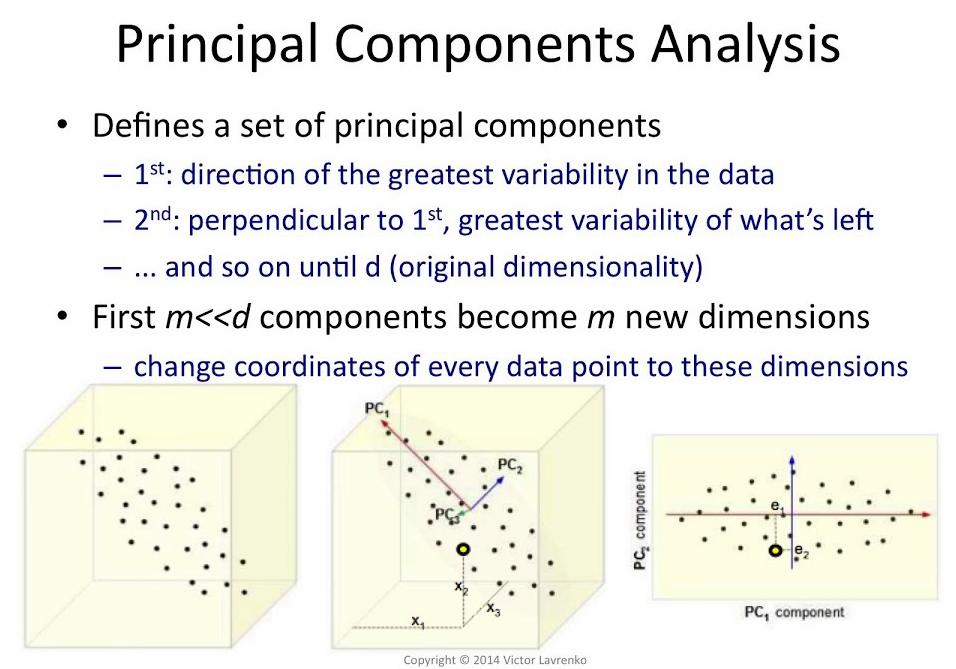
\includegraphics[width = 10cm]{PCA-explanation.jpg}
            \end{figure}

        \clearpage
    \chapter{Clustering}
    \chapter{Regole di Associazione}
    $\textbf{Association Rules}$ è un metodo per l'identificazione di patterns frequenti, correlazioni, associazioni o strutture causali in set di dati.
    \\[1\baselineskip]
    Dato un insieme di transazioni, l'obiettivo dell'Association Rule Mining è trovare le regole che ci consentono di prevedere l'occorrenza di un elemento specifico in base alle occorrenze degli altri elementi nella transazione.
    \\[1\baselineskip]
    Una regola di associazione è normalmente rappresentata nella forma $\{X\} \Rightarrow \{Y\}$ dove:
        \begin{itemize}
            \item $\{X\}$ è la parte $\textit{antecedente}$ (if), ovvero qualcosa che si trova nei dati;
            \item $\{Y\}$ è la parte $\textit{conseguente}$ (then), ovvero qualcosa che si trova in congiunzione con la parte antecedente.
        \end{itemize}

    Un esempio è la seguente frase: "Se un cliente acquista il pane, ha il 70\% di probabilità di acquistare il latte".
    \\
    Il pane è l'antecedente nella regola associativa, mentre il latte è il conseguente.

    \clearpage

    \section{Definizioni}
        Utilizziamo questa tabella per capire meglio le varie definizioni che verranno a breve illustrate:
        
        \begin{figure}[h]
            \centering
            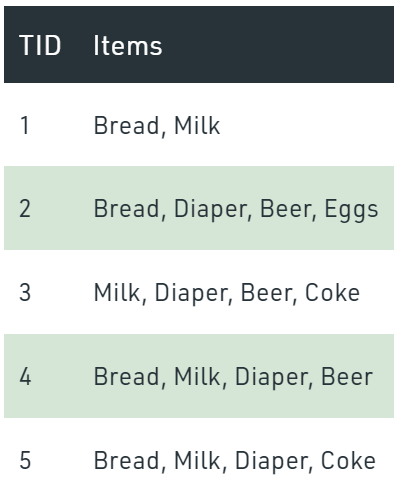
\includegraphics[width = 5cm, height = 4cm]{tabella-supporto-regole-associative.png}
        \end{figure}

        \begin{itemize}
            \item $\textbf{Supporto}:$ annotato come $S \left( X \right)$, è la frequenza di apparizione di $X$ nella tabella.
                Se applicato a una regola, $S \left( X \Rightarrow Y \right)$ è la frequenza di apparizione di $X \cup Y$ e ci indica quante volte appare la regola $X \Rightarrow Y$ nella tabella.
                \\[1\baselineskip]
                Per esempio, $S \left( \textrm{\{Milk, Bread\}} \Rightarrow \textrm{\{Diaper\}} \right) =$
                \\[0.2\baselineskip]
                $\frac{\#(\textrm{\{Milk, Bread\}} \cup \{Diaper\})}{\#\textrm{transazioni}} = \frac{2}{5} = 40\%$.
                \\[0.5\baselineskip]

            \item $\textbf{Confidenza}:$ annotata come $C \left( X \Rightarrow Y \right)$, indica il rapporto tra il numero di volte che appare $Y$ nelle transazioni che includono anche $X$ e il numero di volte che appare $X$.
                \\[1\baselineskip]
                Per esempio, $C \left( \textrm{\{Bread\}} \Rightarrow \textrm{\{Beer\}} \right) = \frac{2}{4} = 50\%$
        \end{itemize}

    \section{Algoritmi}
        \begin{itemize}
            \item $\textbf{Apriori}:$ È utilizzato per la generazione degli itemset frequenti, per approssimazioni successive, a partire dagli itemset con un solo elemento.
                \\[1\baselineskip]
                In sintesi, il presupposto teorico su cui si basa l'algoritmo parte dalla considerazione che se un insieme di oggetti (itemset) è frequente, allora anche tutti i suoi sottoinsiemi sono frequenti, ma se un itemset non è frequente, allora neanche gli insiemi che lo contengono sono frequenti.

            \item $\textbf{FP-Growth}:$ (FP = Frequent Pattern) È un modo alternativo per trovare set di items frequenti senza utilizzare la generazione di candidati, migliorando così le prestazioni.
                \\[1\baselineskip]
                Usa una strategia $\textit{divide et impera}$: il fulcro di questo metodo è l'utilizzo di una speciale struttura di dati denominata Frequent-Pattern Tree (FP-tree), che conserva le informazioni sull'associazione del set di elementi.
                \\[1\baselineskip]
                Usando questa strategia, FP-Growth riduce i costi di ricerca cercando ricorsivamente pattern brevi e poi concatenandoli in dei pattern frequenti più lunghi.
        \end{itemize}

        \begin{figure}[h]
            \caption{Esempio di Apriori}
            \centering
            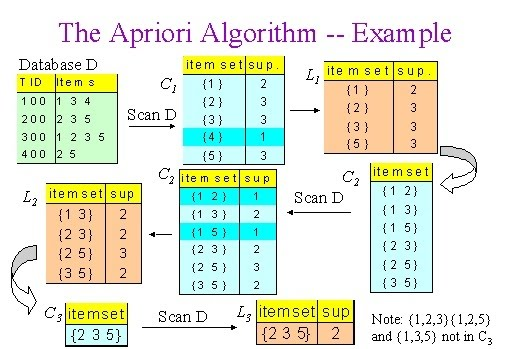
\includegraphics[width = 10cm]{apriori-example.jpg}
        \end{figure}

        \begin{figure}[h]
            \caption{Esempio di FP-Growth}
            \centering
            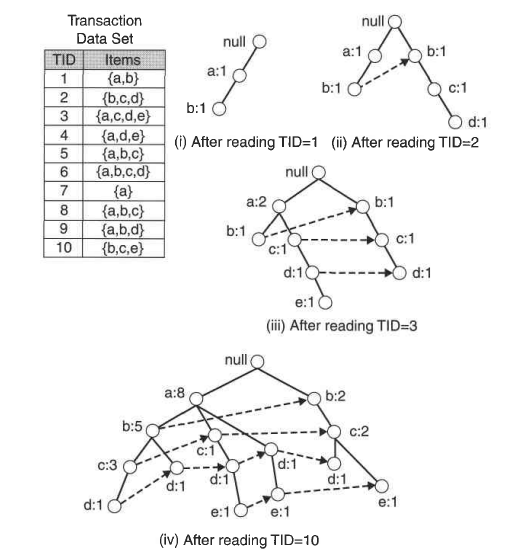
\includegraphics[width = 10cm]{FP-tree-example.png}
        \end{figure}

\clearpage
    \chapter{Recommender Systems}
    Un $\textbf{Recommender System}$ è un sistema di filtraggio delle informazioni che fornisce suggerimenti per gli elementi più pertinenti per un particolare utente (es: film o serie tv suggerite da Netflix).
    
    \section{Misure di Qualità}
        Prima di illustrare i sistemi di raccomandazioni, bisogna fare mente locale su cosa ci serve per capire i vantaggi e svantaggi dei vari sistemi.
        \\[1\baselineskip]
        Per capire ciò, ci si avvale delle $\textit{misure di qualità}$ di un sistema di raccomandazioni.
        Tali misure sono:
            \begin{itemize}
                \item Efficienza nella costruzione del modello;
                \item Efficienza nella generazione dei suggerimenti;
                \item "Serendipity" delle raccomandazioni, ovvero abilità nel suggerire cose non banali e interessanti;
                \item Adattamento al problema della "partenza a freddo" (Cold-Start Problem).
            \end{itemize}

    \section{Sistemi}
        Possiamo identificare ben 3 tipi di recommender systems che utilizzano, ognuno, delle strategie diverse.
        \\
        Prima di tutto, denotando l'insieme degli utenti come $U$ e l'insieme degli items come $I$, formulare il profilo dell'utente $u \in U$ come:
            $$ u = \frac{1}{|I_{u}|} \cdot \sum_{x \in I_{u}}{x}$$

        \subsection{Content-Based}
            Il filtraggio basato sul contenuto utilizza le features degli items per consigliare altri items simili a quelli che piacciono all'utente, in base alle azioni precedenti o al feedback esplicito.
            \\[1\baselineskip]
            La misura di similarità che questo sistema utilizza è il coseno tra due vettori:
                $$ \cos(u, x) = \frac{u \cdot x}{\|u\| \cdot \|x\|} = \frac{\sum_{t}{u[t] \cdot x[t]}}{\sqrt{\sum_{t}{u[t]^{2}}} \cdot \sqrt{\sum_{t}{x[t]^{2}}}} $$

            dove:
                \begin{itemize}
                    \item Ogni item $x \in I$ è un vettore di dimensione $n$, con $n$ che rappresenta il numero di parole nel lessico (creatosi dopo lo stemming, lemming, etc...);
                    \item $x[t] = tf(t, x) \cdot idf(t)$;
                        \\[0.5\baselineskip]
                        $\textbf{Reminder:}$ $\textbf{tf}(t,x)$ è la frequenza del termine $t$ nell'item $x$ e $idf(t)$ è l'invero della frequenza di $t$ nell'insieme di items $I$.
                \end{itemize}

            \subsubsection{Qualità}
                \begin{itemize}
                    \item Facile da costruire in quanto la costruzione di un vettore per ciascuno item non è tanto costoso;
                    \item Non è efficiente nella generazione dei suggerimenti siccome deve cercare i vicini più "vicini" tra tutti i documenti;
                    \item Poca serendipity proprio perché è legato alla similarità del testo di un item;
                    \item Cold-Start Problem "parziale" in quanto un utente dovrebbe prima "toccare" almeno un item.
                \end{itemize}

        \subsection{User-Based}
            Il filtraggio basato sull'utente è una tecnica utilizzata per prevedere gli elementi che potrebbero piacere a un utente sulla base delle valutazioni assegnate a tale elemento dagli altri utenti che hanno gusti simili a quelli dell'utente target.
            \\[1\baselineskip]
            Utilizza una misura di similarità basata su un $\textbf{ranking score}$ $s_{ui}$ dove $u \in U$ e $i \in I$ (indica lo score dell'item $i$ per l'utente $u$):
                $$ s_{ui} = \frac{\sum_{v \in N(u)}{(v[i] - \overline{v}) \cdot \rho(u,v)}}{\sum_{v \in N(u)}{|\rho(u,v)|}} $$

            dove:
                \begin{itemize}
                    \item $\rho(u,v)$ è il $\textbf{coefficiente di correlazione di Pearson}$, usato per pesare il rating di ogni utente $v \in N(u)$ per la similarità tra $v$ e $u$;
                    \item $N(u)$ sono i vicini dell'utente $u$, ovvero un set di utenti simili all'utente target $u$;
                \end{itemize}

            È possibile predire il rating da parte dell'utente $u$ come: $r_{ui} = \overline{u} + s_{ui}$.

            \subsubsection{Qualità}
                \begin{itemize}
                    \item Costoso da costruire in quanto il calcolo della similarità per ogni utente è molto costosa ($O(|U|^{2})$) e deve essere ricomputata per ogni nuovo rating di un utente;
                    \item Efficiente nella generazione dei suggerimenti se la ricerca dei "vicini" viene precomputata offline;
                    \item Ottima serendipity;
                    \item Il Cold-Start Problem è molto problematico perché ha bisogno di un set di ratings sufficientemente grande per ogni nuovo utente/item.
                \end{itemize}

        \subsection{Item-based}
            Il filtraggio basato sull'elemento cerca elementi simili in base agli elementi che gli utenti hanno precedentemente apprezzato o con cui hanno precedentemente interagito positivamente e li consiglia di conseguenza.
            \\[1\baselineskip]
            Utilizza la misura di similarità del coseno, ma aggiustata in modo tale che la misura sia diversa se il set di ratings è diverso
                $$ a-cos(i,j) = \frac{\sum_{u}{(i[u] - \overline{u}) (j[u] - \overline{u})}}{\sqrt{\sum_{u}{(i[u] - \overline{u})^{2}}} \cdot \sqrt{\sum_{u}{(j[u] - \overline{u})^{2}}}} $$

            $\textbf{Nota:}$ il coseno "normale" non è influenzato dalla scala degli elementi/utenti, quindi è come se fossero tutti sulla stessa scala.
                \begin{figure}[h]
                    \caption{A e B sono molto simili ma A è valutato peggio!}
                    \centering
                    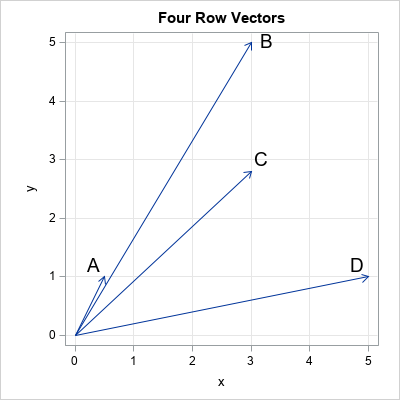
\includegraphics[width = 8cm, height = 6.5cm]{cosine-example.png}
                \end{figure}

            \subsubsection{Qualità}
                \begin{itemize}
                    \item Efficiente da costruire in quanto le computazioni avvengono offline e, generalmente, $|I|$ e più piccolo di $|U|$;
                    \item Efficiente nella generazione dei suggerimenti visto che la ricerca dei vicini più vicini non è necessaria se precomputata offline;
                    \item Meno di quella dello User-Based, siccome il ranking finale dipende dalle ratings dell'utente corrente;
                    \item Il Cold-Start Problem è molto problematico perché ha bisogno di un set di ratings sufficientemente grande per ogni nuovo utente/item.
                \end{itemize}

\clearpage
    \chapter{Shingling \& LSH}

		\subsection*{Premessa}
			Usare il classico algoritmo di ``string matching'' per determinare la similarità fra 2 documenti e' decisamente costoso computazionalmente. Esistono quindi altri metodi di rappresentare un documento che permettono di calcolare la similarità in modi diversi.

	\section{$k$-shingles}
		E' un metodo per la rappresentazione di un documento come un insieme di $k$-grammi, ovvero sottostringhe di lunghezza $k$.

		Costruiti i sottoset di $k$-grammi, si può calcolare la similarità tra due documenti tramite l'indice di Jaccard, ovvero la cardinalità dell'intersezione tra i due insiemi divisa per la cardinalità dell'unione.

		$$
		\text{Jaccard}(A, B) = \frac{|A \cap B|}{|A \cup B|}
		$$

		Tramite questa reinterpretazione, e' possibile avvalorale la similarità fra parole, in modo che pure parole che non sono perfettamente uguali (ad esempio ``player'' e ``players'') possano essere considerate simili.

			\subsection{Come scegliere $k$}
				La metrica $k$ deve essere scelta in base al documento che si vuole rappresentare. Minore e' $k$ e maggiore e' la probabilita' che un particolare $k$-gramma sia presente inoltre cresce la probabilita' che due documenti siano simili.

				E' importante ricordare che il numero di $k$-grammi dipende da $k$ e dalla lunghezza dell'alfabeto usato e cresce esponenzialmente.

				Ad esempio, usando un alfabeto generico di 27 caratteri (26 + spazio), il numero di $k$-grammi e' $27^k$.

	\section{Min-Hashing}
		Sebbene i $k$-grammi forniscano maggiore qualità rispetto al classico ``string matching'', si tratta di una metrica ancora troppo costosa.

		Un metodo abbastanza potente per ridurre notevolmente la dimensione della rappresentazione di un documento è l'uso di un algoritmo di hashing.

		Si consideri un documento $A$ come l'insieme dei suoi $k$-grammi. Il \textbf{min-hashing} di $A$ si definisce come l'elemento più piccolo di $A$ dopo l'applicazione di una permutazione casuale $\pi$. Pertanto il min-hashing di $A$ è dato da un elemento del set scelto casualmente da $\pi$. 

		Applicando la stessa permutazione ad ogni altro documento si ottengono i min-hashing di tutti i documenti.

		\clearpage

		\begin{remark}
			I min-hash dei documenti $A$ e $B$ si denotano come $min(\pi_A)$ e $min(\pi_B)$.
		\end{remark}

		\begin{example}\label{ex:pi_perm}
		$$
		\begin{array}{ccc}
			\begin{array}{ccc}
			& A & B \\ \hline
			a & 1 & 0 \\
			b & 0 & 1 \\
			c & 0 & 0 \\
			d & 1 & 1 \\
			e & 0 & 1 \\
			\end{array}
			\ & \
			\begin{array}{ccc}
			\pi & A & B \\ \hline
			c & 0 & 0 \\
			d & 1 & 1 \\
			b & 0 & 1 \\
			e & 0 & 1 \\
			a & 1 & 0 \\
			\end{array}
		\end{array}
		$$

		La prima tabella rappresenta il documento $A$ e il documento $B$ come insiemi di $k$-grammi. La seconda tabella $A$ e $B$ dopo l'applicazione della permutazione $\pi$.
		\end{example}

		Per calcolare il min-hash dei due documenti è sufficiente scorrere la matrice dall'alto verso il basso seguendo l'ordine della permutazione $\pi$ e prendere la prima riga che contiene un $1$.

		Si nota poi con $x$ il numero di righe in cui entrambi i documenti presentano un $1$, mentre con $y$ il numero di righe in cui \textit{esattamente uno dei due documenti} presenta un $1$. Si scartano quindi le righe in cui entrambi i documenti presentano un $0$.

		Pertanto la probabilità che i due documenti siano simili e che pertanto il loro min-hash sia il medesimo è data dalla probabilità che la prima riga incontrata sia una con $1$ in entrambi i documenti.

		$$ p = \frac{x}{x + y} $$

		\begin{remark}
			Non è strettamente necessario eseguire l'intera permutazione, bensì è sufficiente generare una scelta casuale per la prima riga, scegliendola da quelle contate da $x$ o da $y$.
		\end{remark}

			\subsection{Min-hash Signatures}
				Purtroppo il metodo di min-hash non è così affidabile. Infatti sebbene possa dire che due documenti abbiano una certa probabilità di essere simili, non è in grado di dire quanto siano simili.

				Per superare questa limitazione, si possono usare più permutazioni, quindi calcolare più min-hashes. Supponendo di avere un set di permutazioni 
				$$\pi_1, \pi_2, \dots, \pi_n$$
				si può calcolare la similarità costruendo il vettore

				$$ \left[ \min(\pi_A^1), \min(\pi_A^2), \dots, \min(\pi_A^n) \right] $$

				per ogni documento. Ogni vettore che rappresenta un documento è detto \textbf{signature}. Questo tipo di ``firma'' può essere utilizzato per fornire una stima della similarità tra due documenti.

				Prendendo $k$ il numero di min-hash uguali, calcolate da $m$ permutazioni diverse per $A$ e $B$, allora l'indice di similarità è dato da
				$$ \text{Jaccard}(A, B) \approx \frac{k}{m} $$

				Ovviamente il tradeoff è che più permutazioni si usano e più la similarità è precisa, ma più è costoso il calcolo. In generale si vuole mantenere $m$ inferiore alla media di termini contenuti in un documento.

	\section{Hashing con sensibilità locale (LSH)}
		Pure tramite il min-hashing il costo computazionale può risultare troppo elevato. È necessario un metodo che permetta di eseguire una ricerca più rapida, mantenendo tuttavia un'alta probabilità che se due documenti sono simili, allora il loro min-hash sia lo stesso.

		Per farlo si può suddividere il set di min-hash $m$ in $b$ blocchi di $r=m/b$ elementi ciascuno. Ogni blocco è quindi un vettore di $r$ elementi. Ognuno di essi viene poi concatenato e nuovamente hashato, in modo da ottenere un nuovo vettore detto ``super-signature'' o ``super-shingle''

		In questo modo si salvano i documenti in hash-tables basate sulle super-signatures. Inoltre si utilizzano $b$ tabelle diverse, in modo da mantenere indipendentemente le $b$ super-signatures.

		Il funzionamento dell'algoritmo è il seguente:	
		\begin{enumerate}
			\item Si calcolano le min-hash di un documento $A$
			\item Si calcolano le $b$ super-signatures di $A$
			\item Si usano le super-signatures per accedere alle hash-tables
			\item Si recuperano i documenti associati a tali hash-tables
			\item Si ritorna l'unione di tutti i documenti recuperati
		\end{enumerate}

		Addizionalmente si può in seguito calcolare la similarità fra $A$ e i documenti con l'indice di Jaccard, il quale sebbene sia costoso, verrebbe applicato ad un sotto-set ristretto dei documenti, in modo da filtrare eventuali "falsi positivi".

		\clearpage

		\subsection{Similarity Hashing}
			Si consideri la seguente immagine, nella quale si vedono due documenti $A$ e $B$ come un vettore bidimensionale, dove i due vettori sono separati da un certo angolo $\theta$.

			\begin{figure}[h]
				\centering
				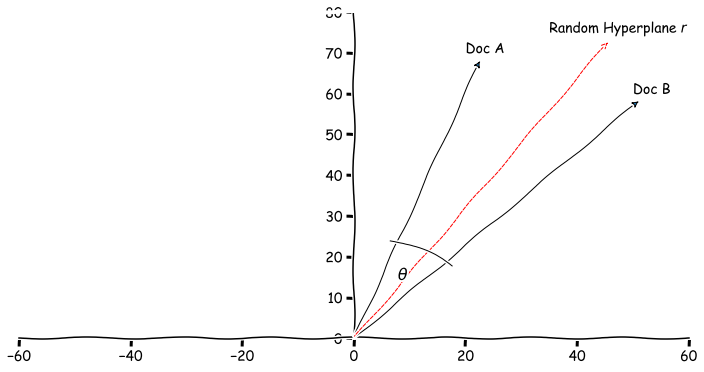
\includegraphics[width=1\textwidth]{images/sim-hash.png}
				\caption{Similarity Hashing}
			\end{figure}

			Preso un vettore casuale $r$ (un iperpiano se fossimo in uno spazio a più dimensioni), qual è la probabilità che $A$ e $B$ siano separati da $r$?

			Ponendo che l'angolo di $r$ può essere compreso fra $[0, 180]$ gradi, allora
			\begin{itemize}
				\item La probabilità che $r$ separi $A$ e $B$ è data da $\frac{\theta}{180}$
				\item Al contrario, la probabilità che $r$ non separi $A$ e $B$ è data da $\frac{180 - \theta}{180}$
			\end{itemize}

			\begin{remark}
				In pratica l'iperpiano $r$ rappresenta una firma composta da un singolo bit per un dato documento. Se il documento è al di sopra dall'iperpiano, allora il bit è $1$, altrimenti è $0$.
			\end{remark}

			Pertanto la probabilità che due documenti abbiano la stessa firma (quindi siano dallo stesso lato rispetto ad $r$) è data da
			$ \frac{\theta}{180} $

			\begin{remark}
				Dato un documento $A$ si può usare la seguente strategia
				
				\begin{enumerate}
					\item Si genera $r$ come una sequenza casuale di $+1$ e $-1$
					\item Si computa il prodotto scalare $r \cdot A$
					\item Se il risultato è positivo, allora si aggiunge un $1$ alla firma, altrimenti un $0$
					\item Si ripete il processo $m$ volte, ottenendo così una firma di $m$ bit
					\item Infine si può sfruttare la distanza di Hamming per calcolare la similarità fra due documenti
				\end{enumerate}
			\end{remark}



\end{document}